% !TEX root = ../main.tex

\chapter{The SBN program at Fermilab and the ICARUS experiment}
\label{chap:icarus_detector}

\section{The Short Baseline Neutrino program at Fermilab}
%% BRIEF INTRODUCTION
The Short Baseline Neutrino experimental program at the Fermi National Accelerator Laboratory (FNAL) aims to  draw a complete and consistent picture of the sterile neutrino scenario, whose anomalies where described in detail in \autoref{chap:theory_introduction}. 
% The main physics goal of the SBN collaboration is to test with great sensitivity the presence of a fourth sterile neutrino state, as suggested by multiple experimental anomalies. 
To achieve a level of statistical significance greater than $5\sigma$ for the LSND-allowed region (at \SI{90}{\percent} CL), SBN will carry out precision searches, recording a neutrino statistics corresponding to \SI{6.6e20}{proton-on-target} during four years of data taking. This is expected to produce approximately one million of neutrino interaction inside the SBN near and far detectors \cite{acciarriProposalThreeDetector2015}. 

The key to such high sensitivity, other than the great statistic of events collected, is the design paradigm of the program. It employs the Liquid Argon Time Projection Chamber (LArTPC) technology \cite{rubbiaLiquidArgonTime1977}, with two functionally identical detectors placed at different distances from the neutrino source. This allows to measure the oscillation pattern by comparing the neutrino flux registered at the far detector with the ``control'' flux recorded at the near detector, reducing the underlying systematic uncertainties related to neutrino production and neutrino interaction cross-sections in argon. 

Albeit the original plan for a three-detector program \cite{acciarriProposalThreeDetector2015}, MicroBooNE collaboration anticipated data taking and the experiment was completed in 2020, two years prior to ICARUS starting its data collection campaign and four prior to SBND, so the SBN program will perform a search for the sterile neutrino as a two-detector experiment \cite{acciarriProposalThreeDetector2015, machadoShortBaselineNeutrinoProgram2019}. 

Both experiments, ICARUS and SBND, collect data from the common Booster Neutrino Beam (BNB) \cite{Stancu:2001cpa}; additionally, the ICARUS detector position makes it sensitive to ${\sim}\SI{6}{\degree}$ off-axis neutrinos coming from the Neutrino at the Main Injector (NuMI) beam \cite{Adamson:2015dkw}. 

ICARUS \cite{abratenkoICARUSFermilabShortBaseline2023} is the far detector for the SBN program, employing an active mass of \SI{476}{\tonne} of liquid argon (LAr), at a distance of \SI{600}{\meter} from the neutrino source; its position was chosen so as to maximise the oscillation probability (see \autoref{fig:oscillation_2body_SBN}; further context is in the next paragraph). ICARUS started its data taking in June of 2022, after the initial commissioning phase. It has now finished the fourth data collection campaign, collecting ${\sim} \SI{7.54e20}{POT}$ (proton-on-target) in total, corresponding to about \num{e6} neutrino events.

Located at a distance of \SI{110}{\meter}, SBND \cite{SBND:2025lha} is the near detector of the SBN program, with an active LAr mass of \SI{112}{\tonne}. After commissioning, it started data taking in December of 2024, jointly with the far detector, thereby allowing the possibility to reduce flux- and cross-section-related systematics. 

\paragraph{Oscillation measurements with a two-detector experiment} The main physics goal of the SBN program is the search for a fourth sterile neutrino state assuming the $3+1$ model. Using multiple LArTPC detectors, a high-sensitivity search for a high-$\Delta m^2$ splitting is possible by studying muon-neutrino oscillations in the $\PGnGm\to\PGnGm$ disappearance and $\PGnGm\to\PGne$ appearance channels  \cite{acciarriProposalThreeDetector2015}. 

\begin{figure}
    \centering
    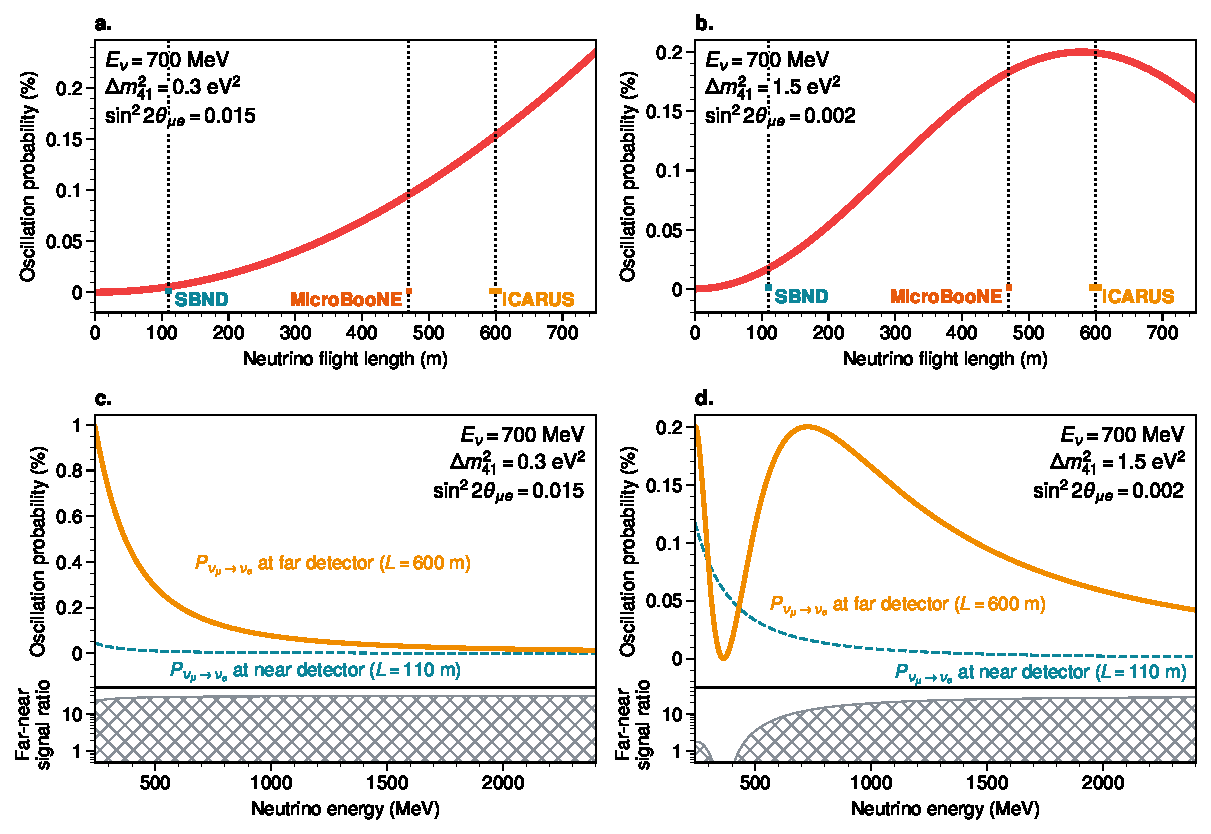
\includegraphics[width=\linewidth]{SBN_sensitivity/appearance_signal.pdf}
    \caption[Electron neutrino appearance probability in the $3+1$ sterile oscillation scenario]{(a) and (b) show the oscillation probability for a \SI{700}{MeV} muon neutrino into an electron neutrino as a function of the length of the neutrino flight using two benchmark values of $(\sin^22\theta_{\PGm\Pe}, \Delta m^2)$. (c) and (d) show the same oscillation probability as a function of the neutrino energy. Additionally, the bottom panels show the far-over-near event ratio. Figure adapted from \cite{machadoShortBaselineNeutrinoProgram2019}.}
    \label{fig:oscillation_2body_SBN}
\end{figure}

The oscillation probability for both channels is presented in Eq. \eqref{eq:2body_oscillation_sterile_disapp} and Eq. \eqref{eq:2body_oscillation_sterile_app} for the disappearance and appearance channels, respectively, within the assumption of the $3+1$ model. Looking at the data in the $\PGnGm\to\PGne$ appearance channel, from the experimental results shown in \autoref{fig:all_experimental_searches}, the allowed parameter space lies in \begin{equation}
    \sin^22\theta_{\PGm\Pe} \in (\num{e-3},\num{e-1})\quad \text{and}\quad \Delta m^2 \in (\num{e-1}, \num{e1})\ \si{eV^2}; 
\end{equation} the location of the near and far detector  has been optimised to maximise the oscillation probability in this region of parameters. \autoref{fig:oscillation_2body_SBN} shows $P(\PGnGm \rightarrow \PGne)$ for two benchmark values of $(\sin^22\theta_{\PGm\Pe}, \Delta m^2)$, assuming a neutrino energy of ${\sim}\SI{700}{MeV}$. 
The choice for a two detector configuration arises from the need to reduce the impact of systematic uncertainties. The strong correlation between the fluxes collected in the near and far detector is key to reducing the impact of some of the major sources of systematic uncertainties, coming from the difficulty in modeling the production mechanism and the $PGn$-Ar interaction cross-sections. 

With a planned collected statistics of \SI{6.6e20}{POT}, both the $\PGne\to\PGne$ as well as the $\PGnGm\to\PGnGm$ disappearance channels can also be probed to search for neutrino oscillation mediated by a sterile state. The unitarity of the $3+1$ PMNS matrix has to be preserved so that in the event of $\PGnGm\to\PGne$ appearance, meaning a nonzero value of $\sin^22\theta_{\PGm\Pe}$, a nonzero value of $\sin^22\theta_{\PGm\PGm}$, or a $\PGnGm\to\PGnGm$ disappearance signature, should be observed. 

All three channels will be studied to either pinpoint the correct $(\sin^22\theta, \Delta m^2)$ values driving short-baseline oscillations or exclude further regions in the parameter space. \autoref{fig:sbn_2det} shows the projected excluded and allowed regions of the parameter space in both the \ref{sub@fig:nue_app_sbn_2det} $\PGne$-appearance and \ref{sub@fig:numu_disapp_sbn_2det} $\PGnGm$-disapperance channels of the two-detector operation of the SBN experiment. It should be noted that the projected \SI{6.6e20}{POT} exposure represents the statistics anticipated in the SBN program proposal \cite{acciarriProposalThreeDetector2015}; however, BNB will operate until 2027, allowing the ICARUS detector to collect three times the statistics in standalone operation. 

\begin{figure}
    \centering
    \subfloat[]{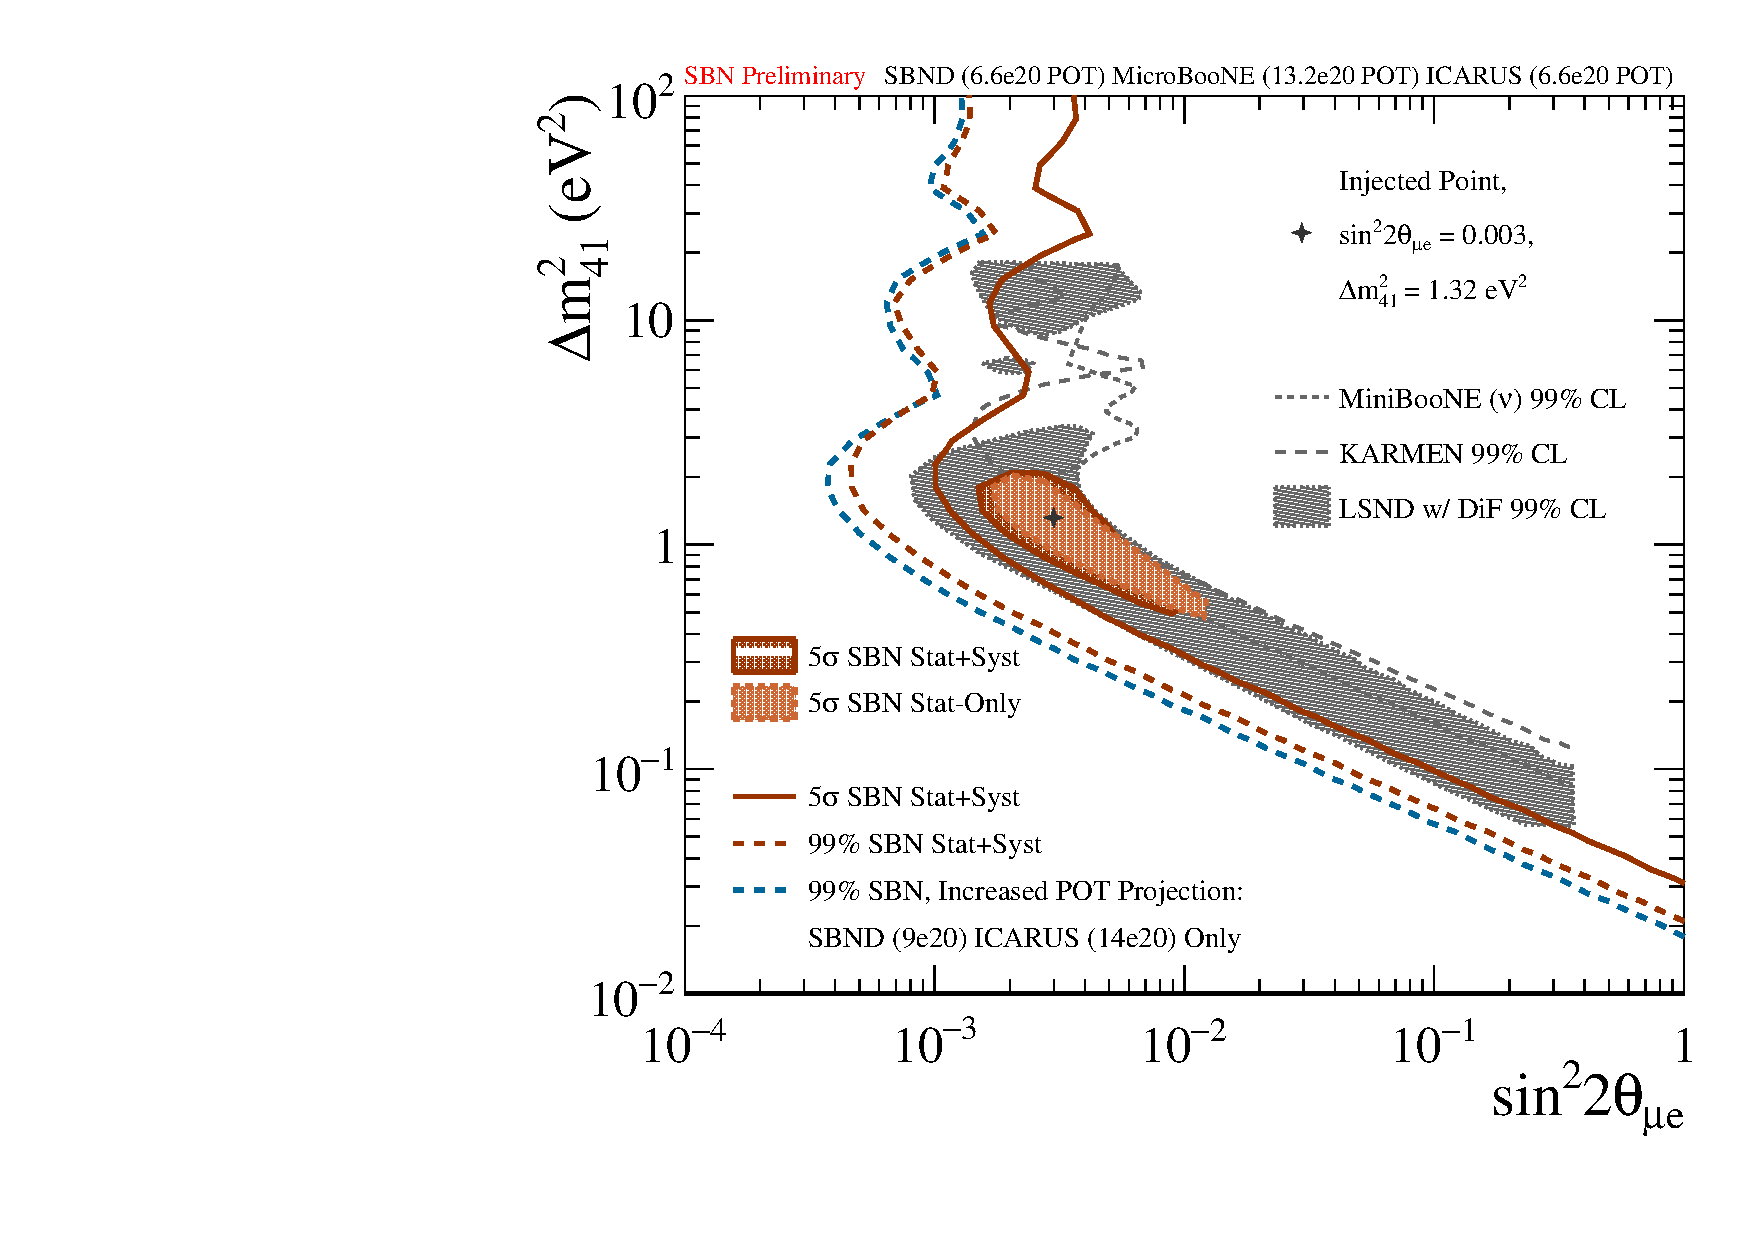
\includegraphics[width=0.5\linewidth]{SBN_sensitivity/nue_app_2det_newPOT_sensitivity_comparison.pdf}\label{fig:nue_app_sbn_2det}}
    \subfloat[]{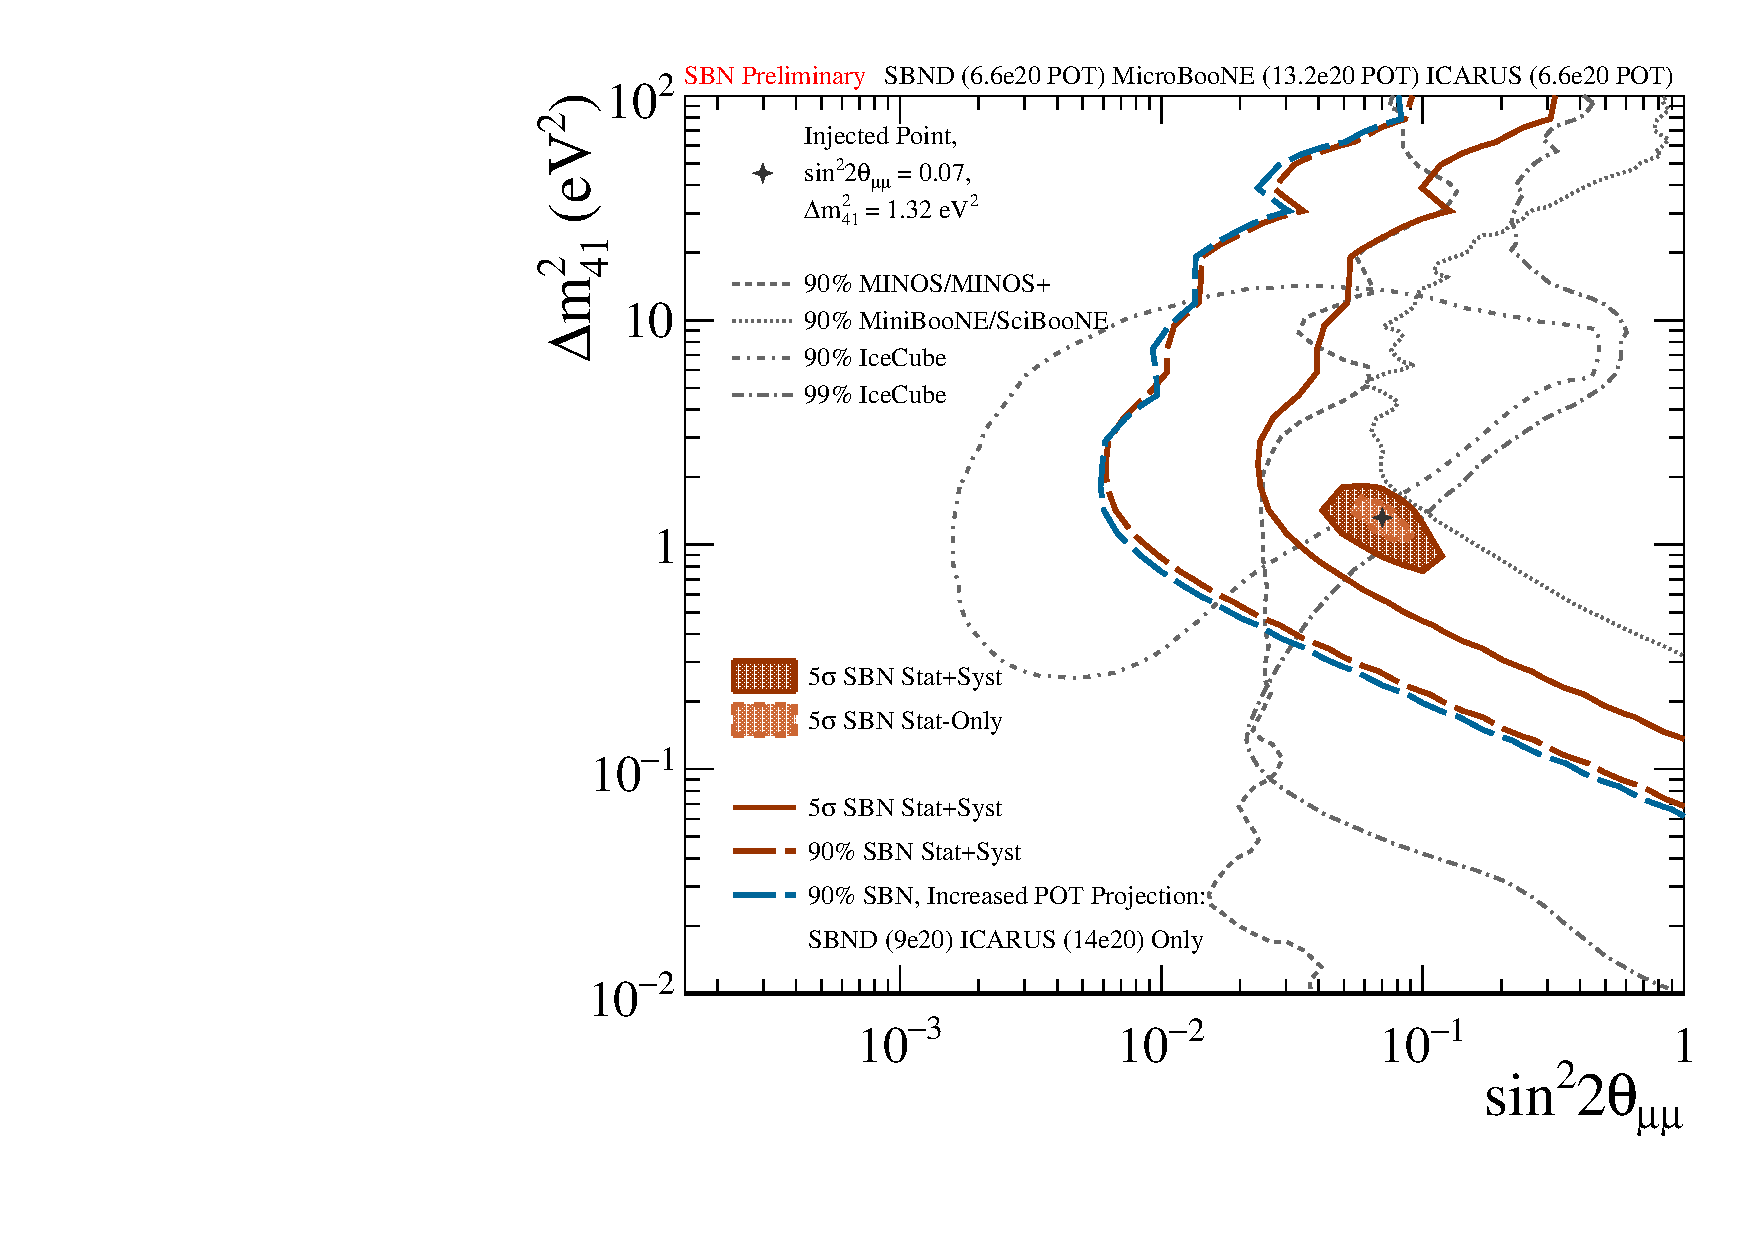
\includegraphics[width=0.5\linewidth]{SBN_sensitivity/numu_disapp_2det_newPOT_sensitivity_comparison.pdf}\label{fig:numu_disapp_sbn_2det}}
    \caption[SBN sensitivity plots in both appearance and disappearance channels]{\ref{sub@fig:nue_app_sbn_2det} and \ref{sub@fig:numu_disapp_sbn_2det} show, respectively, the expected sensitivity exclusion (solid and dashed lines, respectively at $5\sigma$ and 99\% CL) and discovery (filled regions) areas in the $\PGne$-appearance and $\PGnGm$-disappearance channels. These projections account for a collected \SI{6.6e20}{POT} and a two-detector configuration. }
    \label{fig:sbn_2det}
\end{figure}

Additionally, since a nonzero value of both $\sin^2 2\theta_{\PGm\Pe}$ and $\sin^22\theta_{\PGm\PGm}$ leads to a nonzero value of $\sin^22\theta_{\Pe\Pe}$, both the ICARUS detector, making use of the Booster and NuMI neutrino beams, and the SBND detector, only with data from the Booster beam, will explore the $\PGne$-disappearance channel $\PGne\to\PGne$. The combined result of this multi-channel search will provide strong evidence in favour of or against the $3+1$ sterile neutrino scenario. 

\paragraph{Cross-sections and BSM physics} In addition to the primary physics goals, the SBN program, with its two LArTPC detectors, represents a rich opportunity for neutrino physics in general. 

Starting from particle interactions in liquid argon, both SBND and ICARUS detectors will use the Booster and NuMI (ICARUS-only) neutrino beams to perform cross-section measurements, exploiting the great amount of collected data with both detectors. 
For SBND, the proximity with respect to the neutrino source leads to a very large flux collected by the detector --- each run approximately of \SI{2.2e20}{POT} corresponds to 1.5M $\PGnGm$ and \num{12000} $\PGne$s; 
the same events will be measured by ICARUS, which at the moment benefits from a longer data collection period and an accumulated statistic of \SI{7.5e20}{POT} in standalone operation. The larger \SI{476}{\tonne} active LAr mass of the ICARUS detector, compared to the smaller \SI{112}{\tonne} of total LAr mass for the SBND detector, also allows for a larger statistics of fully contained events, where all the final state interactions (FSI) are contained inside the detector active volume, allowing for a better particle identification (PID). 
Additionally, the position of the ICARUS detector allows the collection of neutrinos from the NuMI beam at an off-axis angle of \SI{6}{\degree} with respect to BNB direction. 
The added value of the NuMI beam comes from the energy range it covers. 
Using protons from the Main Injector at an energy of \SI{120}{GeV} \cite{Adamson:2015dkw}, it is able to cover the \qtyrange{1}{3}{GeV} energy range, which overlaps greatly with the DUNE operational energy range. Neutrinos from the NuMI beam will also feature an enriched electronic component from the three-body decay of the kaon component, allowing for precise $\PGne$ cross-section measurements. At the moment of writing, two $\PGnGm$ charged current mesonless cross-section analyses, $\PGnGm\mathrm{CCN>1}\Pp0\PGp$ and $\PGnGm\mathrm{CCN}\Pp0\PGp$, are ongoing. 

Finally, exploiting the tracking and calorimetric power of liquid argon TPCs, with exceptional precision and high-performance event reconstruction capabilities, the SBN program opens up invaluable opportunities for new physics searches \cite{machadoShortBaselineNeutrinoProgram2019, acciarriProposalThreeDetector2015}. 
% Recently the first physics paper by the ICARUS collaboration was published, exploring some of these BSM models involving the scalar sector using data from the NuMI beam \cite{icaruscollaborationSearchHiddenSector2025}. 
Using the off-axis NuMI beam (more informations can be foun on later paragraphs) it is possible to probe the decay of high-energy mesons at high angles with respect to the beam direction, hence opening up to BSM physics searches. This is the case, for example, for the first physics paper published by the ICARUS collaboration at Fermilab, looking at di-muon final state topologies to probe the existence of long-lived particles (LLPs) in kaon decays involving a di-muon FSI, $\PK \to \PGp + \mathrm{LLP}(\to \PGm\PGm)$ \cite{icaruscollaborationSearchHiddenSector2025}. This search was performed using both a selection of fully contained events and non-fully contained events, this latter motivated by the sensitivity to an extra productionmode for heavy QCD axions (``ALPs''). 

\subsection{Neutrino beam}

The location for the SBN program was selected to make use of the already existing accelerator infrastructure at Fermilab. \autoref{fig:accelerator_complex} shows the FNAL accelerator complex schematic overview. This complex provides a powerful beam of neutrinos using protons extracted from the Booster accelerator, core to the operation of the SBN experiment, as well as multiple other particle beams (neutrinos and muons, as well as protons) which are employed in other experiments, such as the NuMI beam, whose main users are the NOvA and the MINOS experiments. 

The common starting point is the Linac (linear accelerator), boosting protons up to \SI{400}{MeV} of energy (or ${\sim}\SI{954}{MeV/c}$ of momentum) using radiofrequency (RF) cavities. Accelerated protons are extracted and boosted to an energy of \SI{8}{GeV} within the Booster ring. 

\begin{figure}
    \centering
    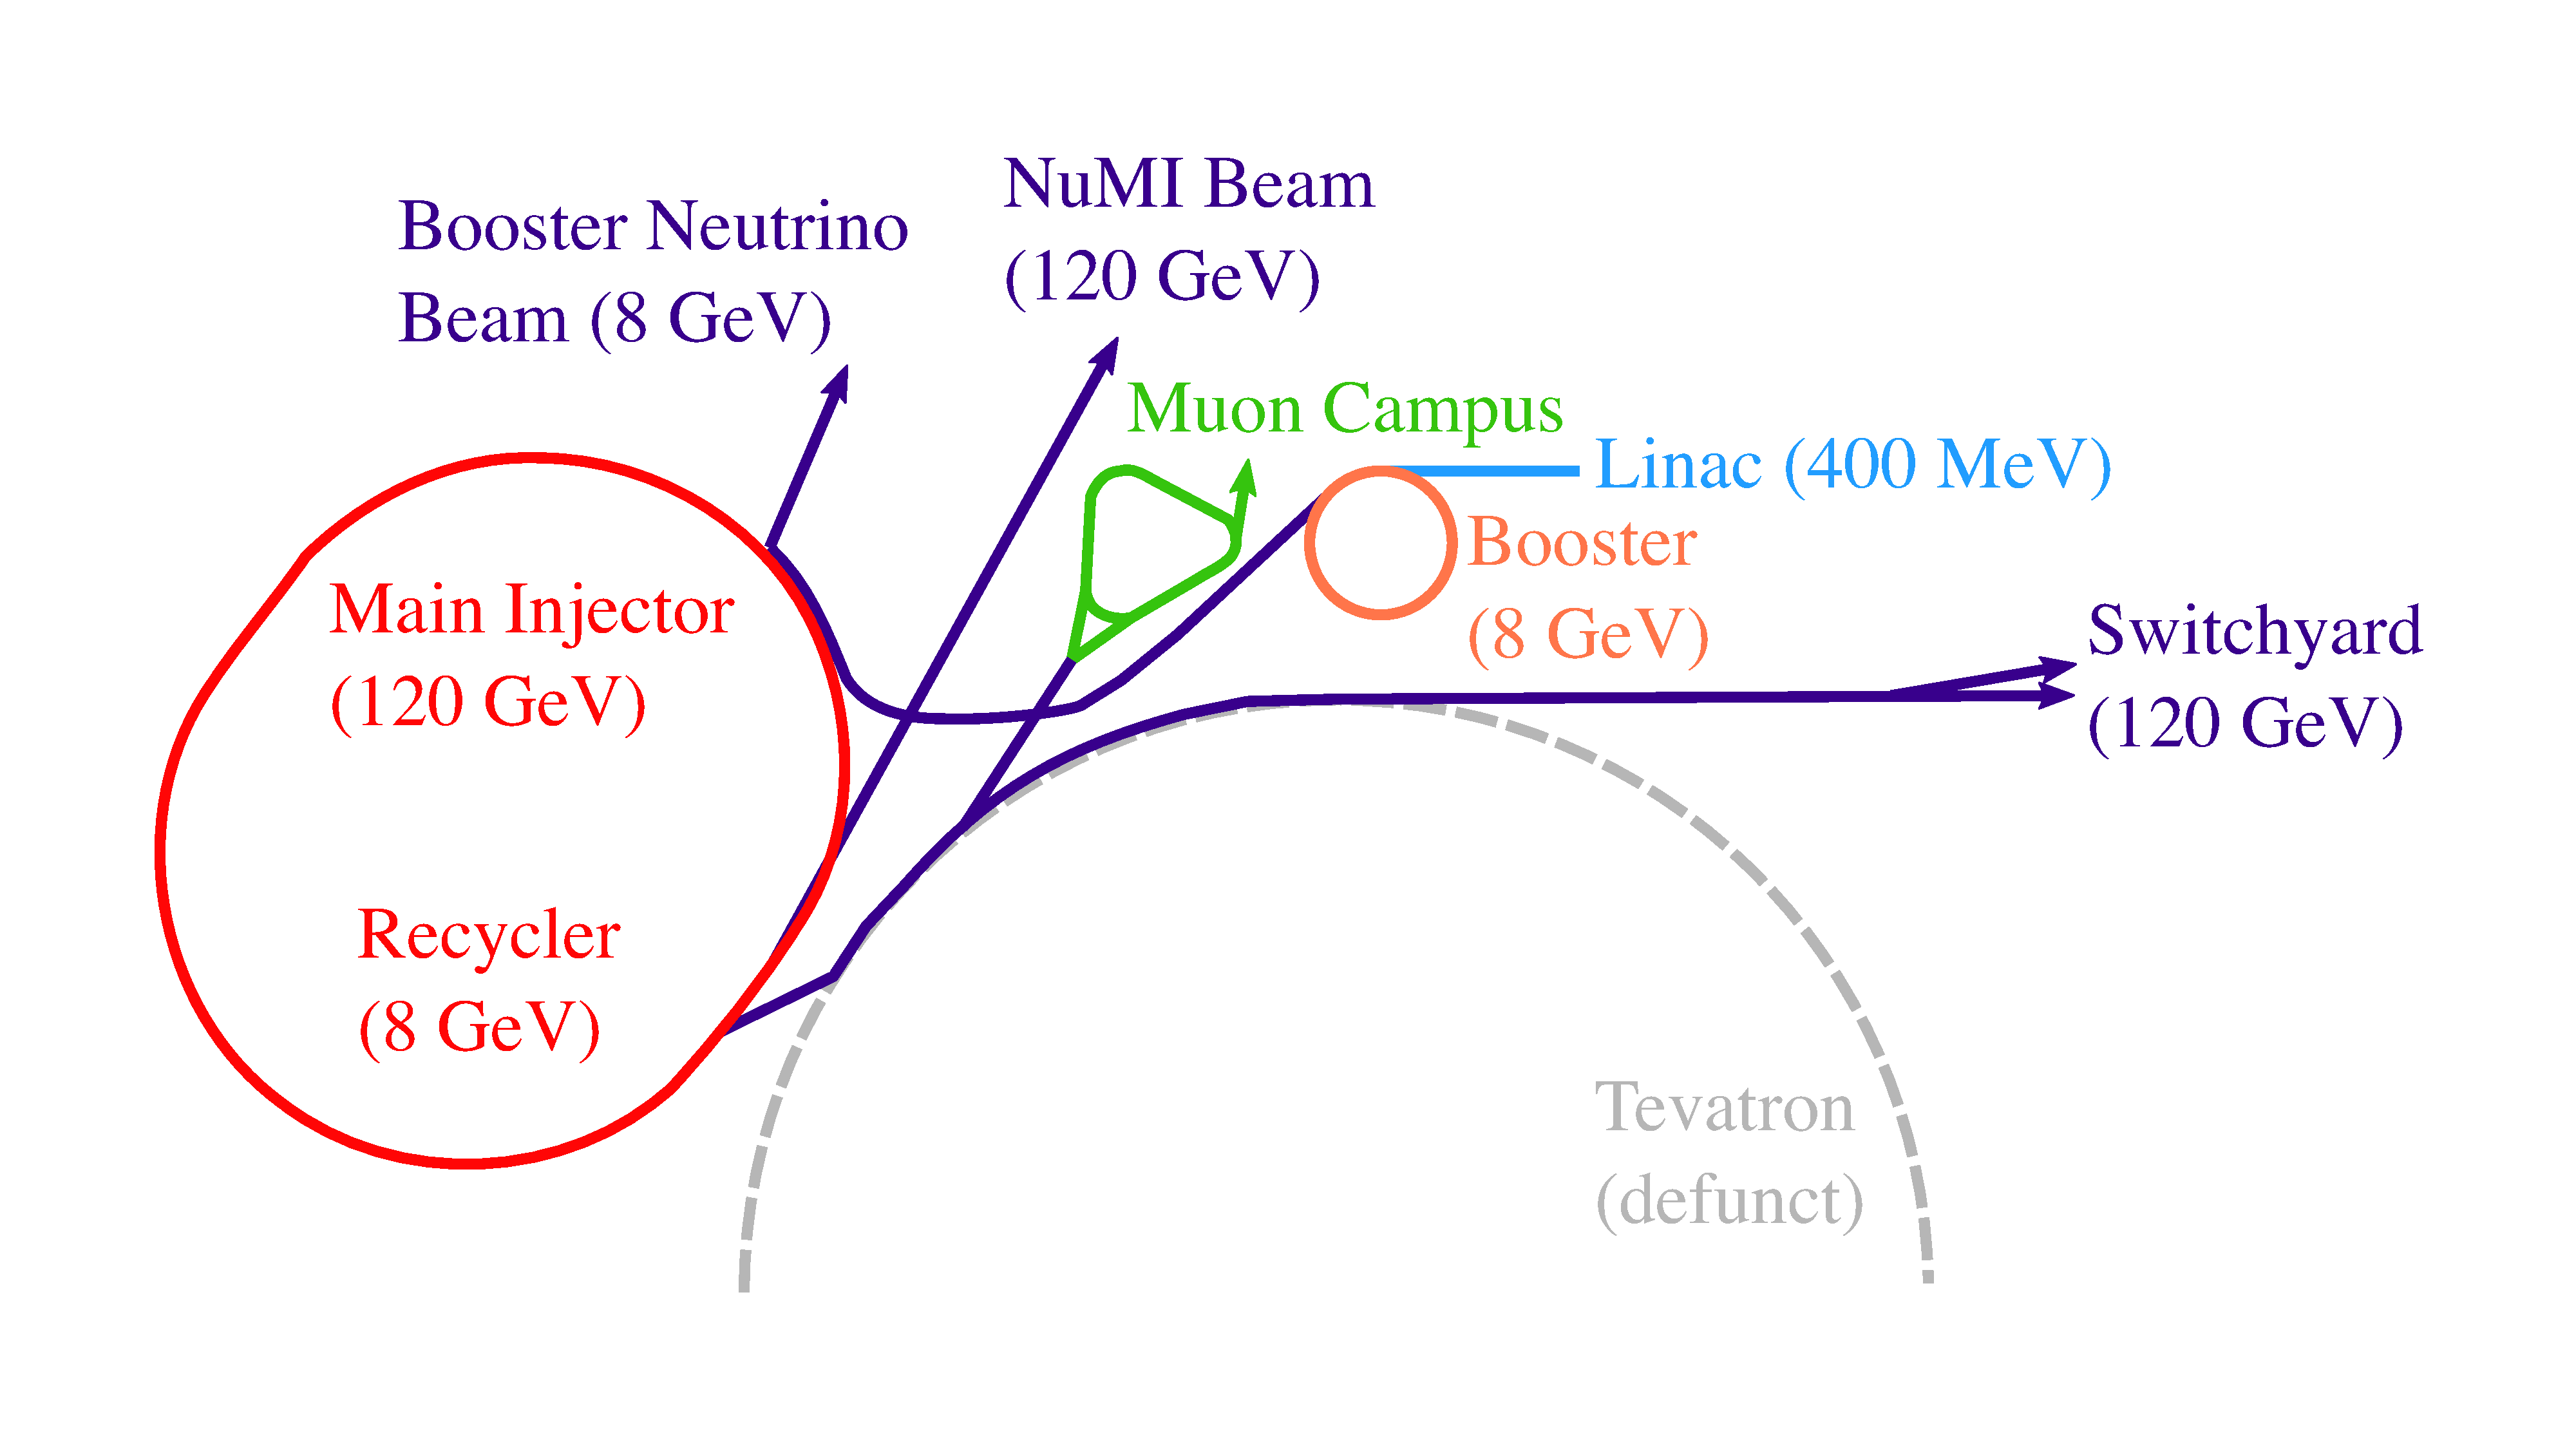
\includegraphics[width=0.75\linewidth]{detector/BNB_NuMI_beams.pdf}
    \caption[Fermilab Accelerator complex]{Schematic representation of the accelerator complex at Fermilab. Both the Booster and NuMI neutrino beams serve the ICARUS detector, covering different energy  ranges, the peak being \SI{700}{MeV} for BNB and \SI{2.5}{GeV} for NuMI. Picture taken from \cite{ainsworthHighIntensityOperation2020}.}
    \label{fig:accelerator_complex}
\end{figure}

From the Booster ring, a fraction of protons is extracted to be used for the Booster Neutrino Beam, whereas the remaining fraction is sent into the Main Injector accelerator. From there a second Neutrino beam is extracted, the Neutrinos at the Main Injector (NuMI) beam. 

\begin{figure}
    \centering
    \subfloat[]{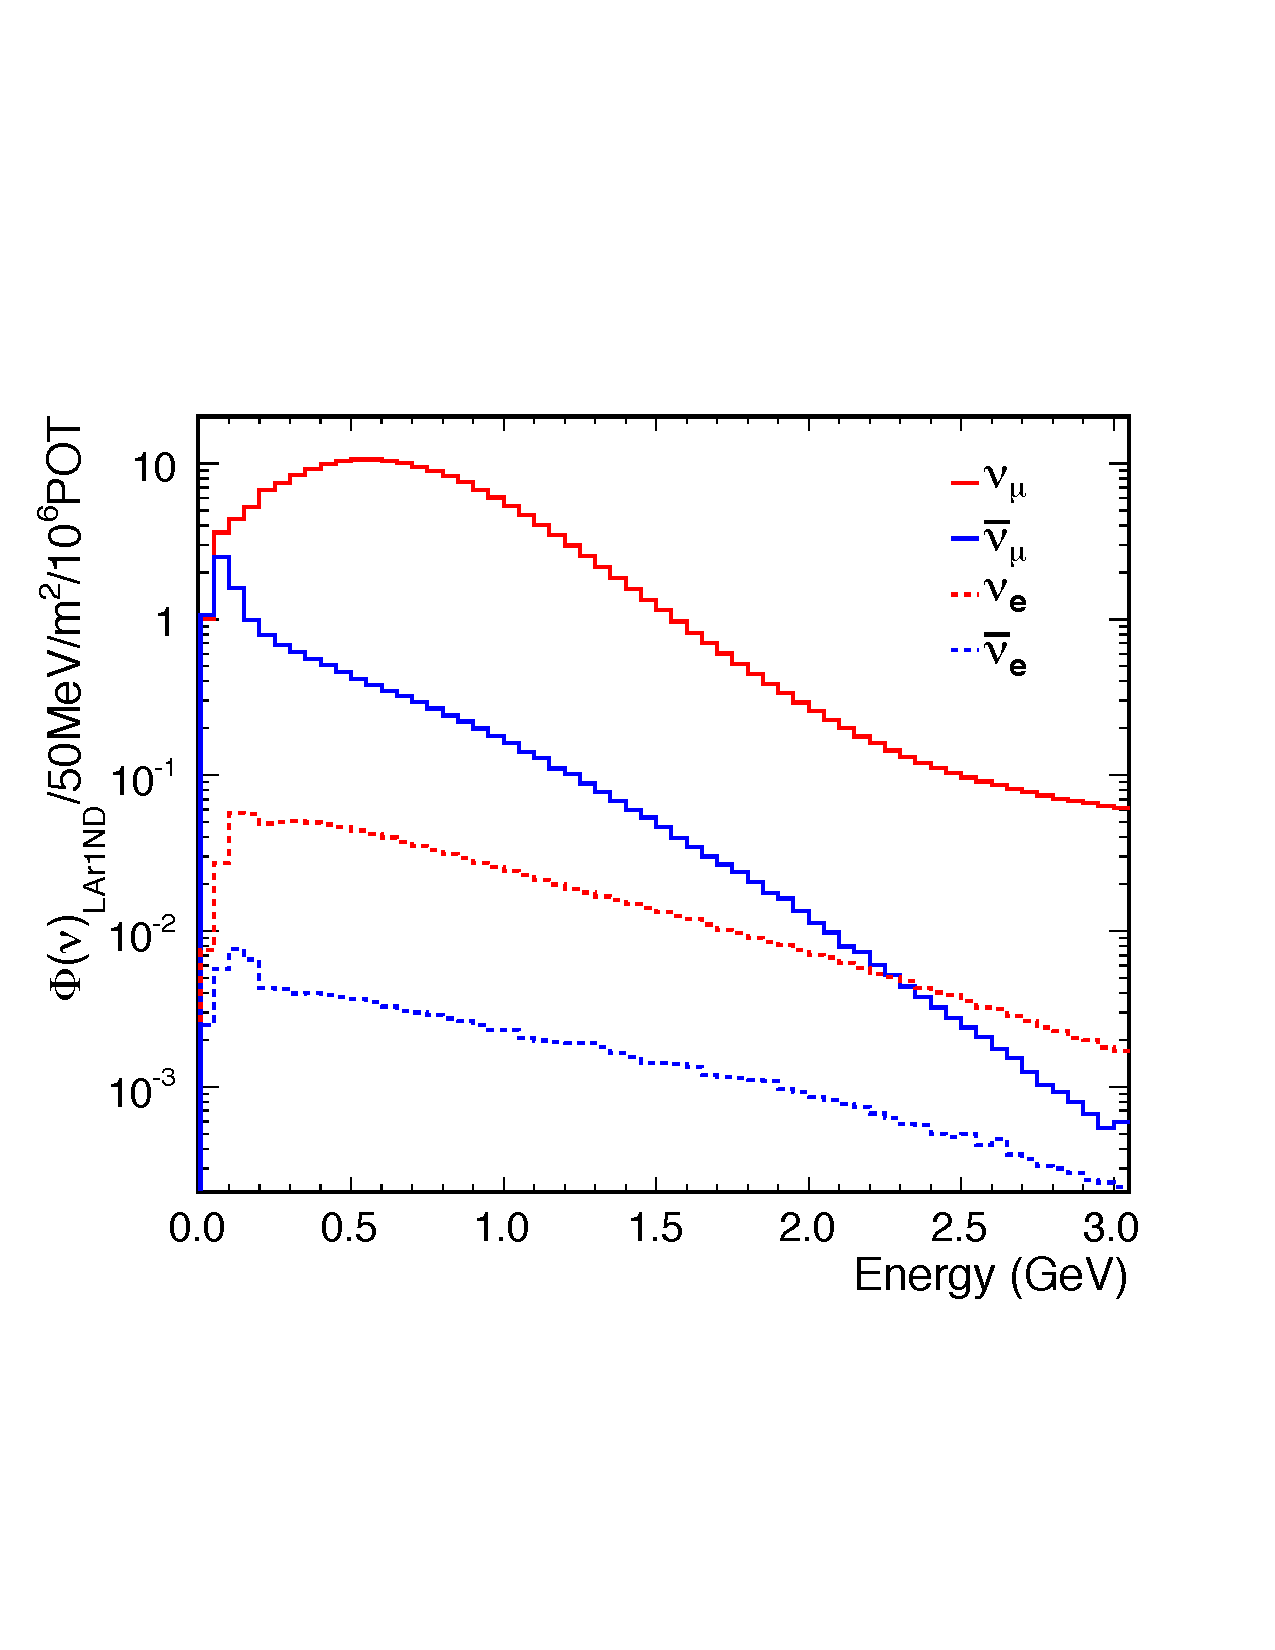
\includegraphics[trim={0 6cm 0 6cm}, width=0.5\linewidth]{beams/BNB_flux_lar1nd.pdf}\label{fig:BNB_flux_SBND}}
    \subfloat[]{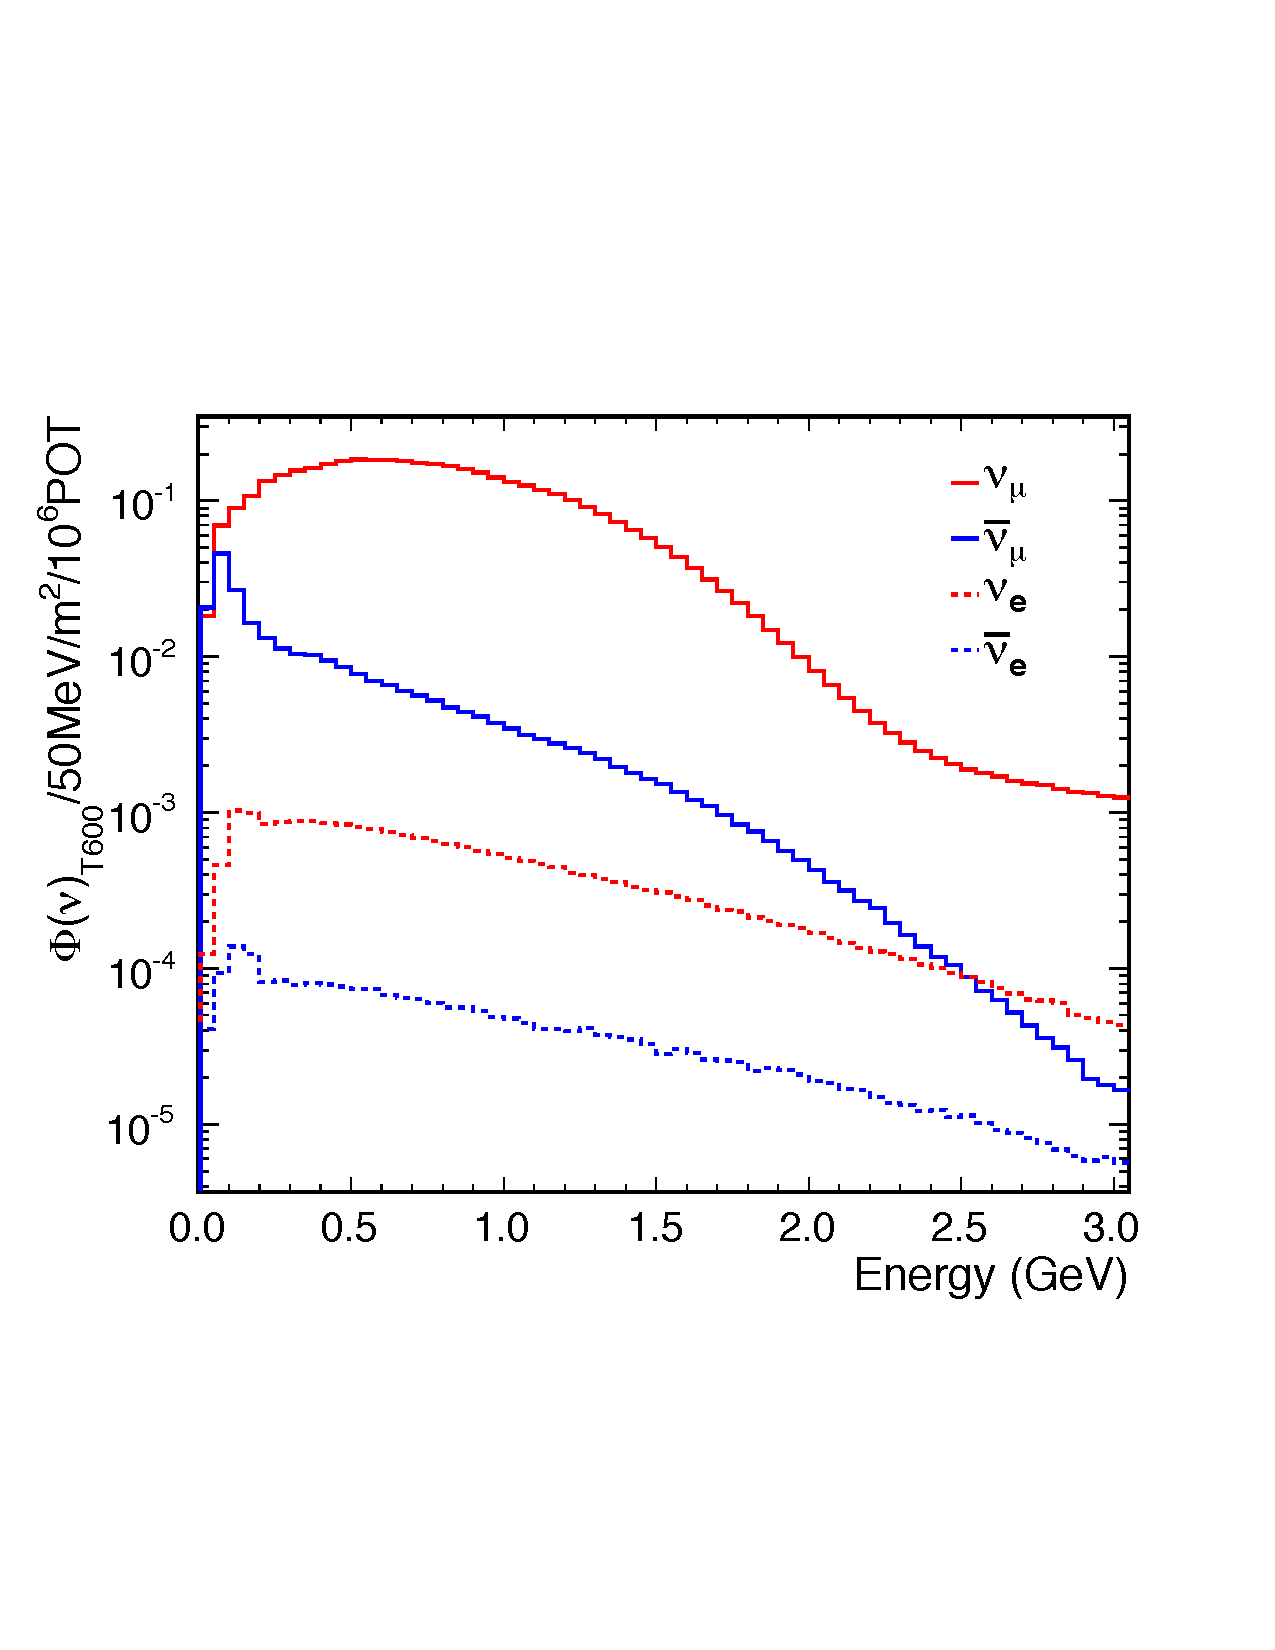
\includegraphics[trim={0 6cm 0 6cm}, width=0.5\linewidth]{beams/BNB_flux_icarus.pdf}\label{fig:BNB_flux_ICARUS}}

    % \subfloat[]{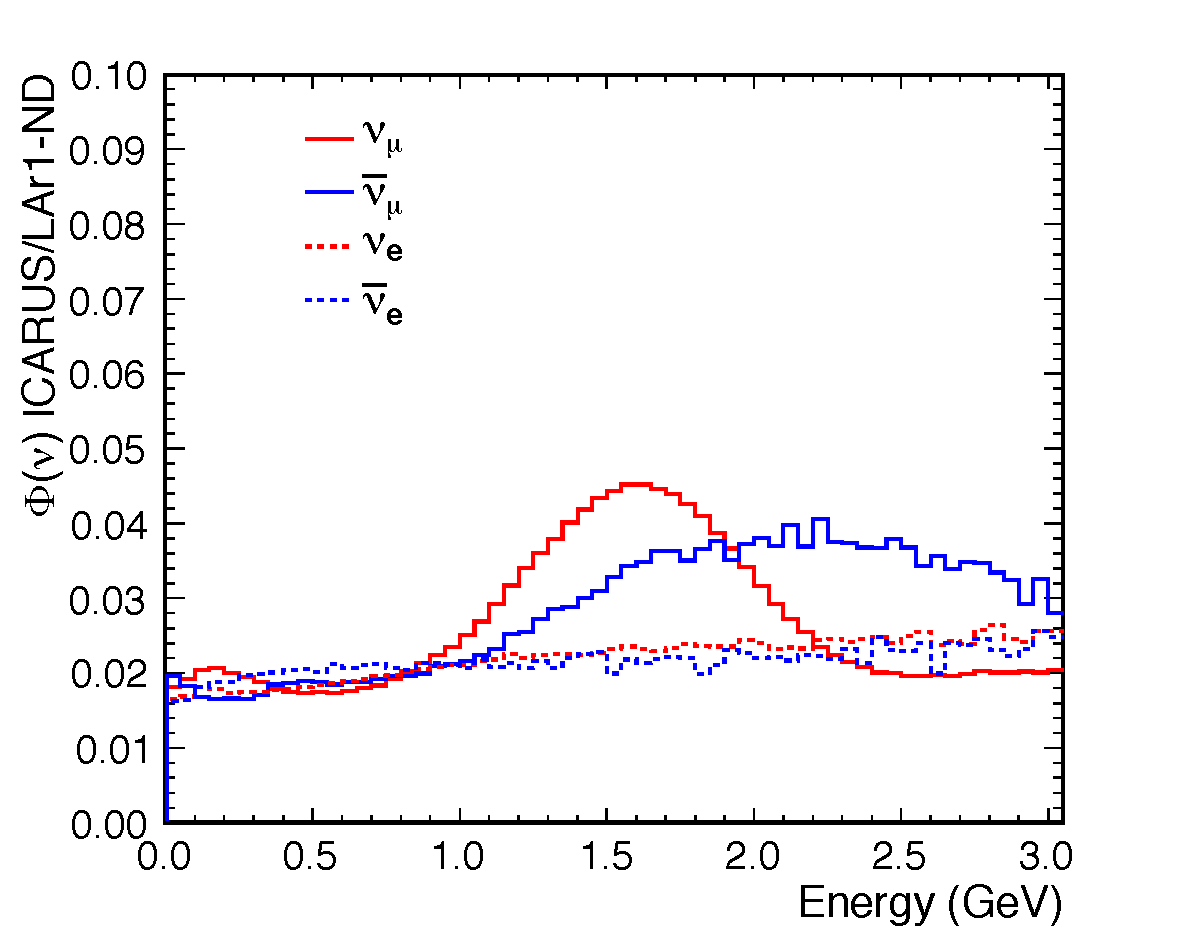
\includegraphics[trim={0 0cm 0 0cm}, width=0.5\linewidth]{thesis/6_figures/beams/BNB_flux_ratio_icarus_lar1nd.pdf}\label{fig:BNB_flux_ICARUS_SBND_ratio}}
    \caption[BNB flux predictions at the near and far detectors]{Predictions of the neutrino flux as computed by the MicroBooNE collaboration \cite{miniboonecollaborationNeutrinoFluxPrediction2009} at distances of \SI{110}{m} \ref{sub@fig:BNB_flux_SBND} and \SI{600}{m} \ref{sub@fig:BNB_flux_ICARUS} from the beryllium target, i.e., for the SBND and ICARUS detectors, respectively. Picture taken from \cite{acciarriProposalThreeDetector2015}. }
    % \ref{sub@fig:BNB_flux_ICARUS_SBND_ratio} shows the predicted ratio of the two fluxes under the hypothesis of no sterile-mediated oscillation anomaly. }
    \label{fig:BNB_flux}
\end{figure}

\paragraph{Booster Neutrino Beam} Protons accelerated up to \SI{8}{GeV} inside the Booster ring are extracted in groups of 81 bunches, each wide ${\sim}\SI{2}{ns}$ and \SI{19}{ns} apart. The repetition rate for the extraction, mainly limited by the focusing horn power supply, is of \SI{5}{\hertz}. Each pulse results in the collision of \SI{5e12}{p} onto a beryllium target, during a beam spill time of \SI{1.6}{\us}. The target is embedded within a pulsed electromagnet (the ``horn'') that produces a toroidal magnetic field to focus positive secondary particles and defocus negative secondary particles emerging from proton-beryllium interactions. Charged mesons, which constitute the majority of the secondary particles emerging from $\Pp$-Be interaction, decay in a 50-meter-long decay region. Within the decay region, charged pions undergo weak decay \begin{equation}
    \PGppm \to \PGmpm + \brabar\PGnGm, \label{eq:pion_decay}
\end{equation} resulting in an (anti)neutrino beam. The length of the decay pipe was chosen so as to maximise the muon (anti)neutrino content and minimise the electron (anti)neutrino content coming from the decay of secondary muons \begin{equation}
    \PGmpm \to \Pepm + \brabar \PGnGm + \brabar \PGne \label{eq:muon_decay}
\end{equation} at ${\sim} \SI{0.5}{\percent}$ level. Neutrinos produced by BNB have a most probable value for the energy at $E_\PGn\simeq \SI{700}{MeV}$, and a maximum energy around \SI{2.5}{GeV}. When the beam is in FHC (forward horn current, selecting primarily positive mesons) mode, its composition is dominated by muon neutrinos ${\sim}\SI{93.6}{\percent}$; the second major component is given by $\PAGnGm$ coming mainly from non-defocused $\PGpm$ \eqref{eq:pion_decay} and decaying muons \eqref{eq:muon_decay}; the same decay accounts for, together with neutral kaon decays, an intrinsic ${\sim}\SI{0.5}{\percent}$ fraction of $\PGne + \PAGne$. 

A detailed study of the beam profile and composition, to allow for its precise simulations, was performed by the MiniBooNE collaboration \cite{miniboonecollaborationNeutrinoFluxPrediction2009}, and experimentally verified using the Hadron Production Experiment (HARP). \autoref{fig:BNB_flux} shows the beam fractional composition as a function of the energy of the neutrino. 

\paragraph{Neutrinos at the Main Injector off-axis beam} Once protons are accelerated within the Booster ring, they are then transferred inside the Main Injector ring. There protons are accelerated up to an energy of \SI{120}{GeV}. The MI circumference is roughly seven times larger than that of the Booster ring, so it can hold up to seven entire Booster cycles in it. However, to make space for the pulse kicker rise time, only six are filled, adding up the spill time to \SI{9.5}{\micro\second}: in such time window, NuMI is able to provide a flux of \SI{6.5e13}{POT}. Protons then collide against a graphite target, and produce mesons that decay inside a \SI{675}{\meter} long decay tunnel. As for BNB, the main decay products are \eqref{eq:pion_decay} muons and muon neutrinos, with a small fraction of muon antineutrinos and electron neutrinos. 

ICARUS is, however, detecting neutrinos from NuMI at an off-axis angle of ${\sim}\SI{6}{\degree}$ with respect to the detector $z$ coordinate, corresponding to BNB direction. This changes the composition of the beam detected by ICARUS, as off-axis neutrinos and antineutrinos have pretty much the same flux, and overall the fraction of electron (anti)neutrinos is larger. This different beam composition, added to the fact that the energy range is higher than BNB energy range, peaking at \SI{1.5}{GeV} and extending up to \SI{4}{GeV}, allows NuMI to be crucial for ICARUS operations: higher energies overlap better with the expected energy spectrum of future experiments, as for example the DUNE experiment, whilst a greater fraction of electron neutrinos allows for the study of both muon- and electron-neutrino argon interaction cross-sections. 
% Additionally, off-axis detection is core for BSM physics searches since it allows to probe the decay of high-energy mesons at high angles with respect to the beam direction. This is the case, for example, for the first physics paper published by the ICARUS collaboration at Fermilab, looking at di-muon final state topologies to probe the existence of long-lived particles (LLPs) in kaon decays involving a di-muon FSI, $\PK \to \PGp + \mathrm{LLP}(\to \PGm\PGm)$ \cite{icaruscollaborationSearchHiddenSector2025}. 

\section{Liquid Argon Time Projection Chambers} 

Core to the high sensitivity of the SBN program is the shared Liquid Argon Time Projection Chamber technology between the two functionally identical near and far detectors. The Time Projection Chamber technology was first proposed by David R. Nygren \cite{Marx:1978zz}. This technology, whose working principle (in this case, of a Liquid Argon TPC, which is the technology employed in the ICARUS experiment) is pictured in \autoref{fig:TPC}, allows both 3D reconstruction as well as calorimetric capabilities. The basic idea of a TPC detector is that of a large volume, filled with gas or liquid, acting as the interaction medium. Charged particles interact inside this volume, producing ionisation pairs. Free electrons produced in the ionisation process are drifted by means of a strong electric field from the cathode toward the anode, where the ionisation electron charge information is collected by a position-sensitive plane, providing one or more 2D projections of the interaction. The drifting time is used as the third missing component to perform 3D event reconstruction inside the detector. 

\begin{figure}
    \centering
    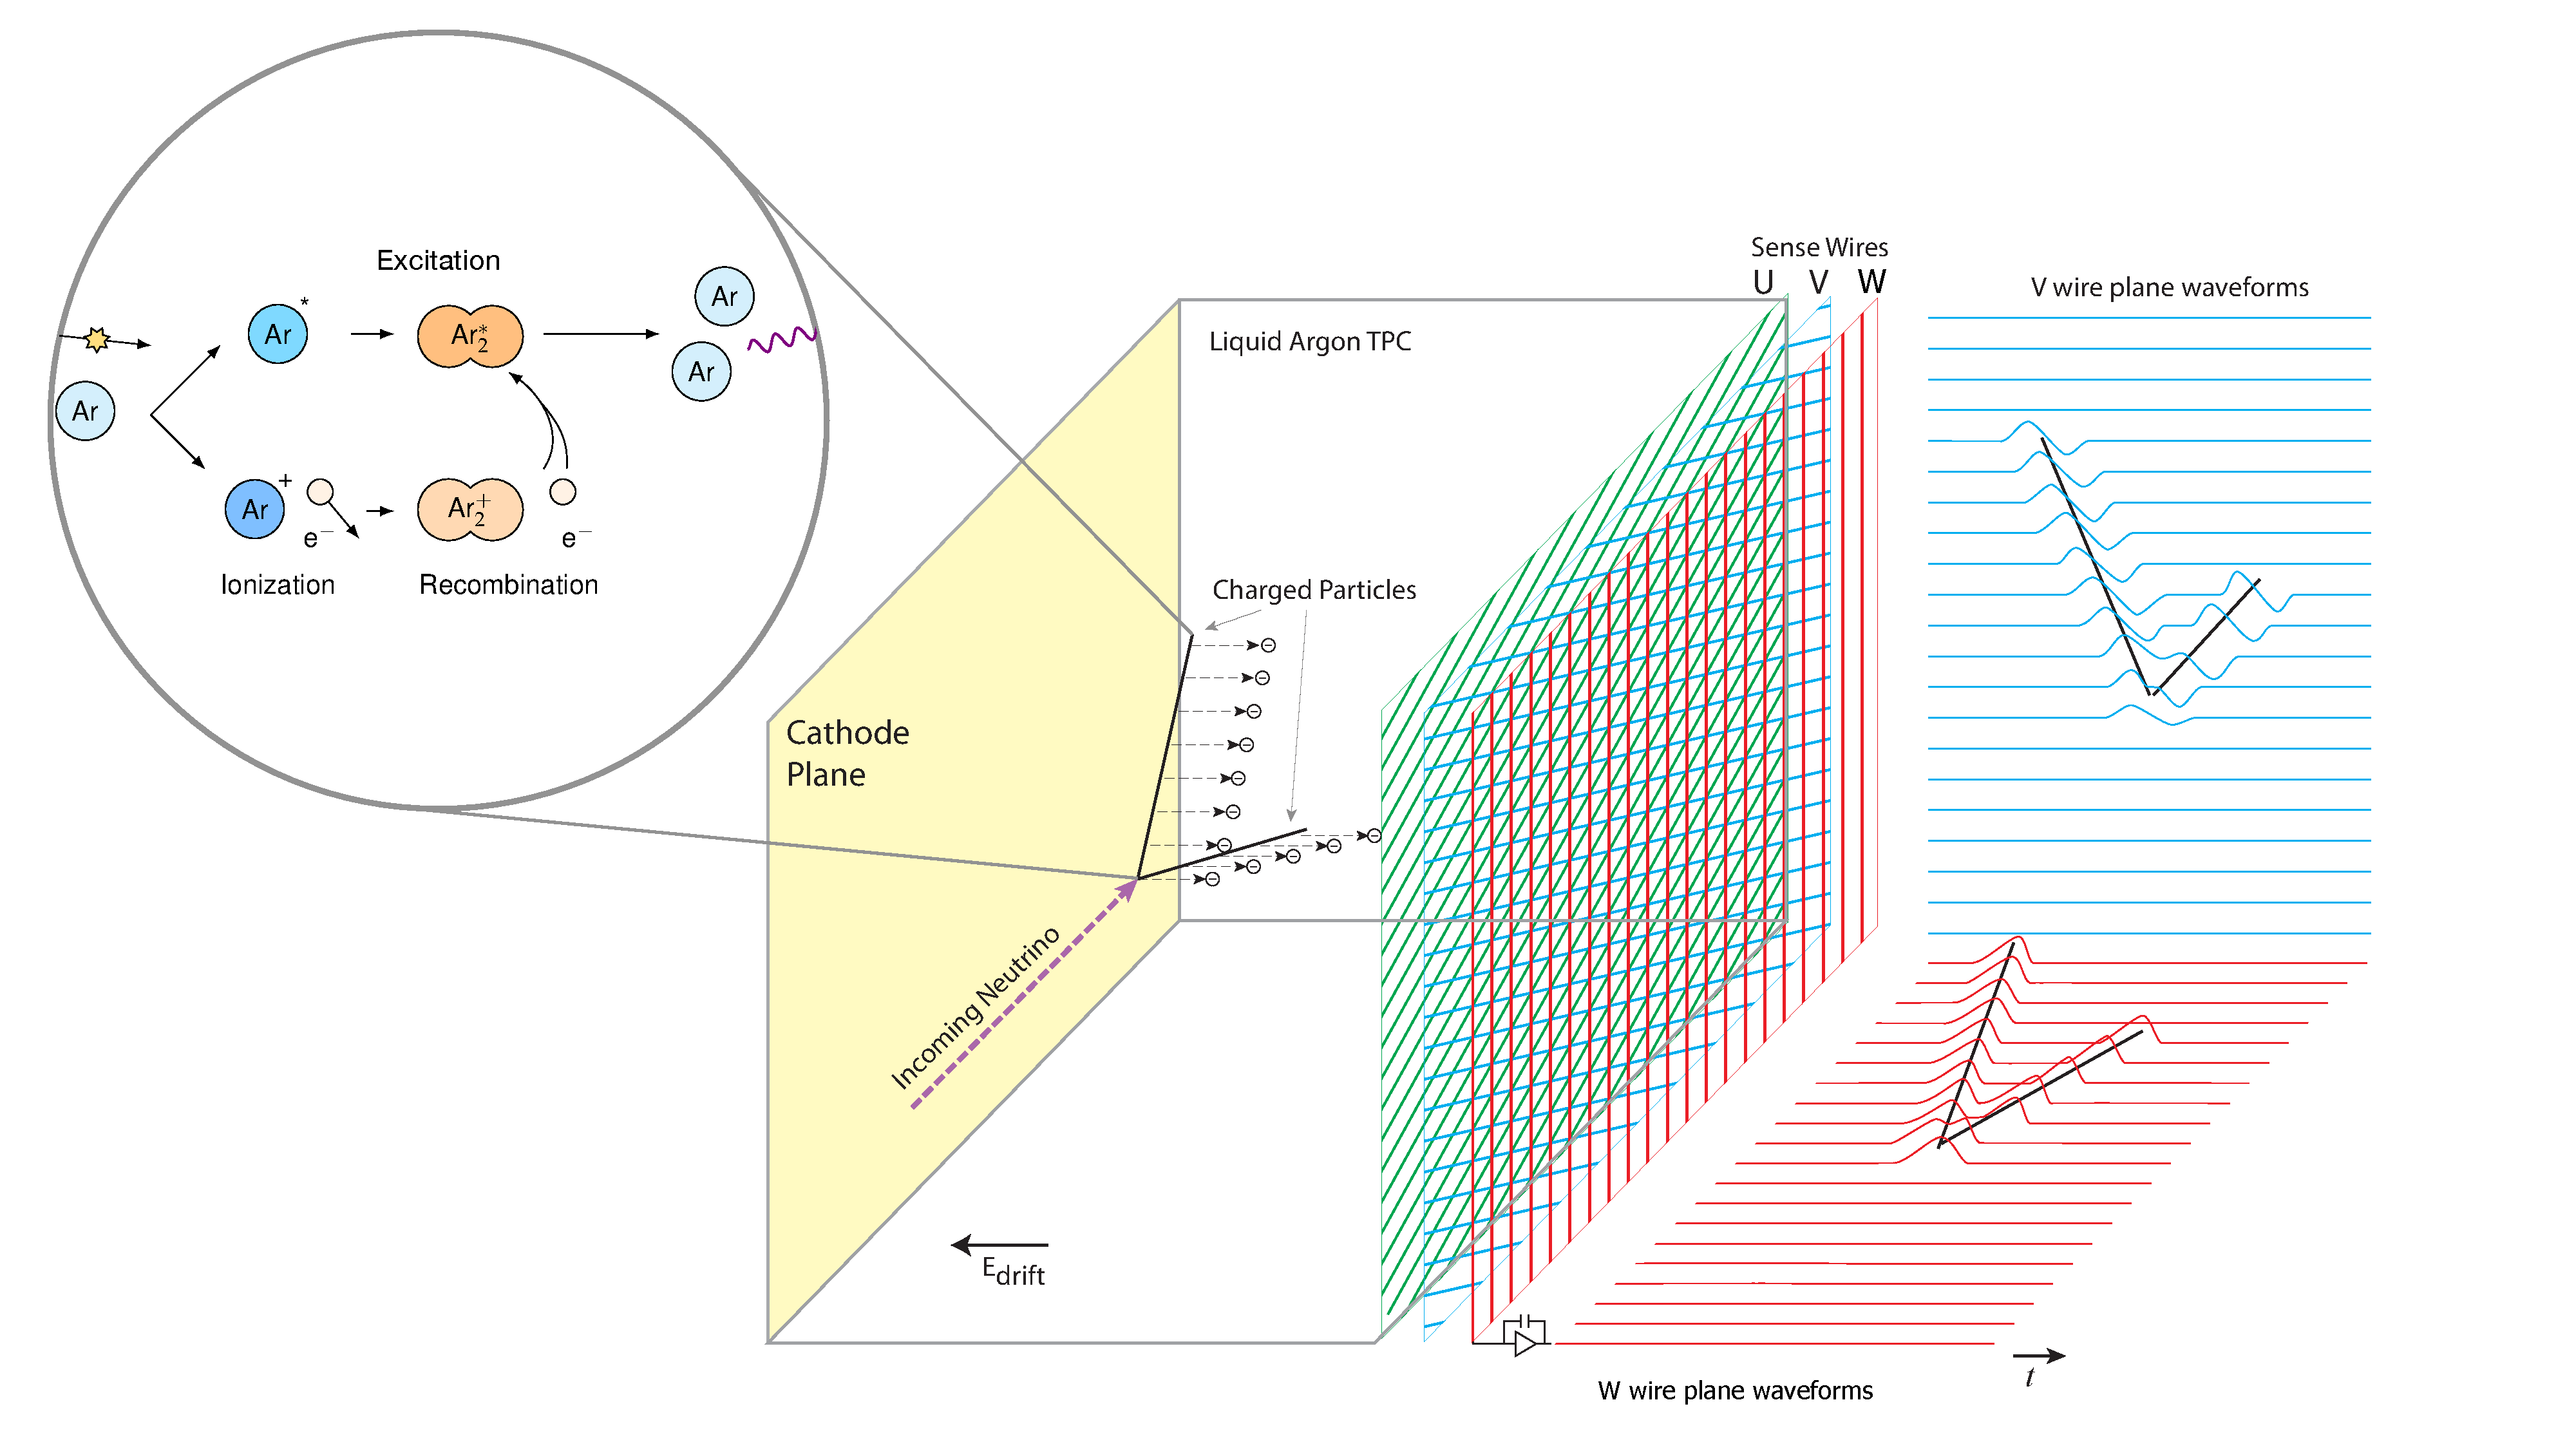
\includegraphics[width=\linewidth, trim={0 0 1.5cm 0}]{detector/TPC_argon.pdf}
    \caption[LArTPC illustration]{Illustration of the working principle of a LArTPC detector. Once neutrinos undergo weak interaction, they ionise the material, producing a large quantity of free electrons that are drifted towards the wire planes. Image adapted from \cite{triozziStudyTriggerSystem}. }
    \label{fig:TPC}
\end{figure}

The first TPCs were built primarily for high energy physics (HEP) applications, and many are still in use for major experiments, such as the ALICE tracker \cite{Lippmann:2014lay}. Carlo Rubbia proposed using liquid argon (LAr) as an interaction target for a TPC, thereby inventing the LArTPC concept for neutrino detection \cite{rubbiaLiquidArgonTime1977}. Liquid argon is an attractive material for particle detection, especially for neutrino physics, given its physical properties \begin{enumerate}
    \item LAr has a high density of \SI{1.39}{\gram\per\centi\meter\cubed} and a high atomic mass, which, combined with the small cross-section of $\PGn$-Ar interaction, allows for more probable detection than most gases.
    \item Being argon a noble gas, it does not attach free electrons, allowing for a longer drift lifetime.
    \item It has high electron mobility, $\mu\simeq \SI{320}{\centi\metre\squared\per\volt\per\second}$ for $E\simeq\SI{0.5}{\kilo\volt\per\centi\metre}$ and $T=\SI{87}{\kelvin}$, allowing for fast drift velocity $v=\mu E \simeq \SI{1.6}{\metre\per\milli\second}$.
    \item The LAr radiation length $X_0\simeq\SI{14}{\centi\metre}$ allows mm-scale calorimetry sampling of neutrino events while having a precise discrimination between electron- and photo-induced electromagnetic showers. Photons produced at the primary vertex usually show a greater conversion gap between the interaction and the starting points of the EM shower; additionally, photo-induced electromagnetic showers display an ionisation pattern in the first centimetres of the shower development compatible with two minimum ionising particles (MIP), whereas electron-induced showers show a pattern compatible with a single MIP \cite{Farnese:2015kfa}.
    \item At the same time, Ar is both easy and cheap to extract. In Earth's atmosphere, it is the third most abundant gas, and can be liquified using nitrogen: this allows for great scalability required to use it for large-scale detectors.
    \item LAr boiling temperature of \SI{87.3}{\kelvin} causes most organic impurities to be frozen out to very low levels. This increases the drift electron lifetime. 
\end{enumerate}

Inside a LArTPC, once the neutrino undergoes weak interaction, it produces secondary charged ionising particles. These in turn ionise LAr nuclei, creating $\mathrm{Ar^+},\ \Pem$ ionisation pairs and producing scintillation light. Roughly \SI{42000}{e} are produced for each MeV of deposited energy\footnote{This number is dependent on the electric field strength inside the detector. This value is the reference with a nominal electric field of ${\sim} \SI{500}{\volt\per\centi\meter}$.}, which are then drifted by means of an electric field toward the anodes. At the anode three planes of wires are placed in sequence, referred to as induction-1 (I-1), induction-2 (I-2) and collection (C) planes. The planes are properly voltage biased to achieve a nearly perfect transparency of the first two wire planes (I-1 and I-2) with respect to the drift electrons, enabling them to induce a charge signal on the first two planes and only be collected by the third plane. Given a nominal electric field inside the detector $E$, a good ``transparency'' of the successive wire planes to the drifting electrons is obtained by requiring that $E_2\geq F\times E_1$, and $E_1 \geq F \times E$ --- where $E_1$ and $E_2$ are respectively the field values in the I-1 to I-2 gap and I-2 to C gap --- with the scaling factor $F\in(1.2, 1.5)$. Due to the ionisation charge inducing a current on the first two planes and depositing the charge only on the third, the signal collected by the three sets of wires is intrinsically different: on the first two, the signal is bipolar, whereas on the third plane, the signal is unipolar. 

The three planes have their wires oriented at different angles to be able to  collect different ``projections'' of the same interaction happening inside the detector. Using this information, it is possible, in the reconstruction stage, to obtain a $\mathcal O(\si{mm^2})$-precision $(y,z)$ image of the interaction. The third $x$ coordinate is reconstructed using the timing information. In fact, when charged particles cross LAr, aside from creating ionisation pairs, they produce scintillation light, which constitutes a prompt signal used to assign the $t_0$ information. Therefore, the missing coordinate is reconstructed by comparing the time at which the electron is recorded on the wire with the prompt scintillation reference time $t_0$, and knowing the drift velocity of ionisation electrons inside LAr, $x = v_\mathrm{d}\times (t - t_0)$. 

Contributing to the formation of scintillation light within LAr are two processes, pictured in the inset of \autoref{fig:TPC} \begin{itemize}
    \item excitation of Ar followed by the formation of the excimer state $\mathrm{Ar_2^*}$, which decay with the production of scintillation photons, \begin{equation}
        \mathrm{Ar^* + Ar} \to \mathrm{Ar_2^*} \to \mathrm{2Ar}+\PGg;
    \end{equation}
    \item recombination of ionized argon atoms with a free electron, especially frequent with clouds of $\Pem$ around ionized $\mathrm{Ar^+}$ nuclei, \begin{equation}
        \mathrm{Ar^++Ar} \to \mathrm{Ar_2^+}\Pem \to \mathrm{Ar_2^*} \to \mathrm{2Ar}+\PGg;
    \end{equation}
\end{itemize}

These two processes combined at cryogenic temperature produce \num{20000} monochromatic vacuum ultraviolet (VUV) photons per MeV of deposited energy, with a wavelength of $\lambda = \SI{128}{\nano\metre}$. This light presents two components, one so-called ``fast'', with a characteristic time $\tau{\sim}\SI{6}{\nano\second}$, and one ``slow'', $\tau{\sim}\SI{1.5}{\micro\second}$ components. Scintillation light is crucial, as already mentioned, for precise determination of the interaction time, required for the trigger system to operate and to reconstruct the third coordinate. Additionally, as will be briefly discussed in \autoref{chap:event_reconstruction}, scintillation light is core for double-checking the $(y,z)$ positioning of the interaction, providing the so-called ``light barycenter''. 

It should be noted, however, that aside from all the aforementioned LAr properties, there are some drawbacks to the use of LAr for particle detection. First and foremost, a complete understanding of the $\PGn$-Ar interaction has not been reached yet, so there are large systematic uncertainties related to the parametrisation of the interaction cross-section. Secondly, in order to keep argon in its liquid phase and minimise the organic impurities, a huge effort is required for the design of the cryogenic infrastructure. Impurities lower the lifetime of drifing electrons in the TPC, making difficult to reconstruct the full charge deposited by the particles in the interaction. ICARUS, during its data taking period at LNGS, reached a record high purity of \SI{20}{ppb} equivalent of $\mathrm{O_2}$ impurities, corresponding to a lifetime of the electron of \SI{16}{\ms} \cite{antonelloExperimentalObservationExtremely2014}.

Whilst this latter problem is intrinsic to the LArTPC design and requires ad hoc designs and implementations of the cryogenic infrastructure to be optimised, the former problem is addressed in the SBN program by using two functionally identical LArTPC detectors, which allows the cancellation of many systematic uncertainties when performing a joint oscillation analysis \cite{acciarriProposalThreeDetector2015}. 

Finally, even though LAr was chosen for its large electron mobility, LArTPCs are intrinsically slow detectors, with drift times of the order of milliseconds. Hence, detectors operating at shallow depth, like ICARUS and SBND, during the readout time window record significant cosmic activity. This reason led both the SBND and ICARUS collaborations to design the detectors to include an external cosmic ray tagger detector system (CRT) with nearly complete $4\pi$ coverage to veto most of the cosmic activity. The cosmic activity during a spill gate of \SI{1.6}{\ms} is expected to be of \numrange{8}{12} cosmic-rays for the ICARUS experiment and \numrange{1}{3} for the SBND experiment.  

\section{The SBN near detector: SBND} 

The Short Baseline Near Detector (SBND) is the near detector of the SBN program at Fermilab. Located \SI{110}{\metre} from the proton-beryllium interaction target and containing \SI{112}{\tonne} of liquid argon, SBND data will provide precise measurements of unoscillated neutrinos spectrum. As a ``flux monitor'', SBND will greatly reduce the impact of systematic uncertainties related to neutrino interactions in argon and also, due to the two detectors being functionally identical, the systematic uncertainties related to the event reconstruction. Following nearly a decade of design, construction, and installation, SBND began its commissioning phase in July 2024, commencing the collection of stable BNB data at an unprecedented rate of approximately \num{7000} neutrino events per day in December 2024 \cite{SBND:2025lha}. 

As for the ICARUS experiment, the physics goals of the SBND collaboration extend beyond the search for eV-scale sterile neutrinos; making use of its huge statistics, due to its proximity to the beam source point, SBND will allow for extremely precise $\PGn$-Ar interaction cross-section measurements in both the sub-GeV and GeV energy ranges. Additionally, the proximity to the neutrino source point allows the detector to cover both the on-axis as well as the off-axis phase space for BNB, expanding its capabilities to BSM physics studies similar to the ones performed by ICARUS collaboration using NuMI beam data. 

SBND's LarTPC consists of a single module, with dimensions of $\qtyproduct[product-units = power]{5x4x4}{\meter}$, holding a total mass of \SI{112}{\tonne} of LAr. The structure contains two TPCs sharing two common cathode plane assemblies (CPAs) positioned at the centre and parallel to the beam direction, and four anode plane assemblies (APAs) at the other two ends. The maximum drift length for the SBND detector is \SI{2}{\meter} which, for the nominal electric field of \SI{500}{\volt\per\cm}, leads to a maximum drift time of \SI{1.3}{\ms}. Each APA holds three planes of wires spaced \SI{3}{\mm} apart from each other, each hosting \num{2816} wires oriented at \SI{+-60}{\degree} (I-1/$u$ and I-2/$v$, respectively) and \SI{0}{\degree} with respect to the vertical $y$ axis. 

The photon detection system (PDS) of SBND was developed to enhance the light collection and at the same time test relevant technologies for future generation experiments such as DUNE. The first task is addressed by making the cathode reflective and also coated in TPB, thereby allowing the light shifted from VUV to ${\sim}\SI{400}{\nm}$ where PMTs operate to be collected with increased efficiency. The second item for SBND's PDS was addressed by adopting two different light collection systems, PMTs, as for many other LArTPCs, and X-ARAPUCA. These are new innovative light collection technologies developed for the present and future detectors like ProtoDUNE and DUNE, adopting the silicon photomultiplier technology for light collection \cite{Bonivento:2024qpn}. 

The SBND detector finished its commissioning phase last summer and since then has started collecting physics data alongside the ICARUS detector for use in the SBN program. 

\section{The ICARUS-T600 detector}  \label{sec:ICARUS_T600}

The ICARUS (Imaging Cosmic And Rare Underground Signals) detector, the far detector for the SBN program, with an active mass of \SI{476}{\tonne} of liquid argon, is the first ever large-scale operating LArTPC detector \cite{amerioDesignConstructionTests2004c}. It consists of two identical adjacent T300 modules with internal dimensions \qtyproduct[product-units = power]{3.6x3.9x19.6}{\meter}. Each T300 module houses two adjacent LArTPCs separated by a common cathode, with a maximum drift distance of $\simeq\SI{1.5}{\m}$, equivalent to a drift time of ${\sim}\SI{1}{\ms}$ for a nominal \SI{500}{\volt\per\cm} electric drift field.

The cathode is built up by an array of nine panels made of punched stainless steel, allowing for a \SI{58}{\percent} optical transparency between the two drift regions. The anode plane assemblies are made of three parallel wire planes, spaced \SI{3}{\mm} apart; each plane holds \SI{150}{\um} thick stainless steel wires oriented on each plane at different angles with respect to the horizontal direction. The wire orientation for the planes in the ICARUS detector is quite unique with respect to other operational LArTPCs. For both TPCs in a T300 module, the Induction-1 wires are at \SI{0}{\degree}. The orientation of the  Induction-2 and Collection planes is different for the East and West TPC in each T300 module as shown in \autoref{fig:i2_c_planes_wirepitch_detail}. For the East anode planes in both East and West cryostats, Induction-2 is oriented at \SI{+60}{\degree} and Collection at \SI{-60}{\degree}, whereas for the West anode planes, their orientation is reversed, with I-2 at \SI{-60}{\degree} and C at \SI{+60}{\degree}. With this design, as illustrated in the images on both sides of \autoref{fig:i2_c_planes_wirepitch_detail}, electrons drifting from either TPC ``see'' the wires in both the I-2 and C planes as identically oriented \cite{amerioDesignConstructionTests2004c}. 

\begin{figure}
    \centering
    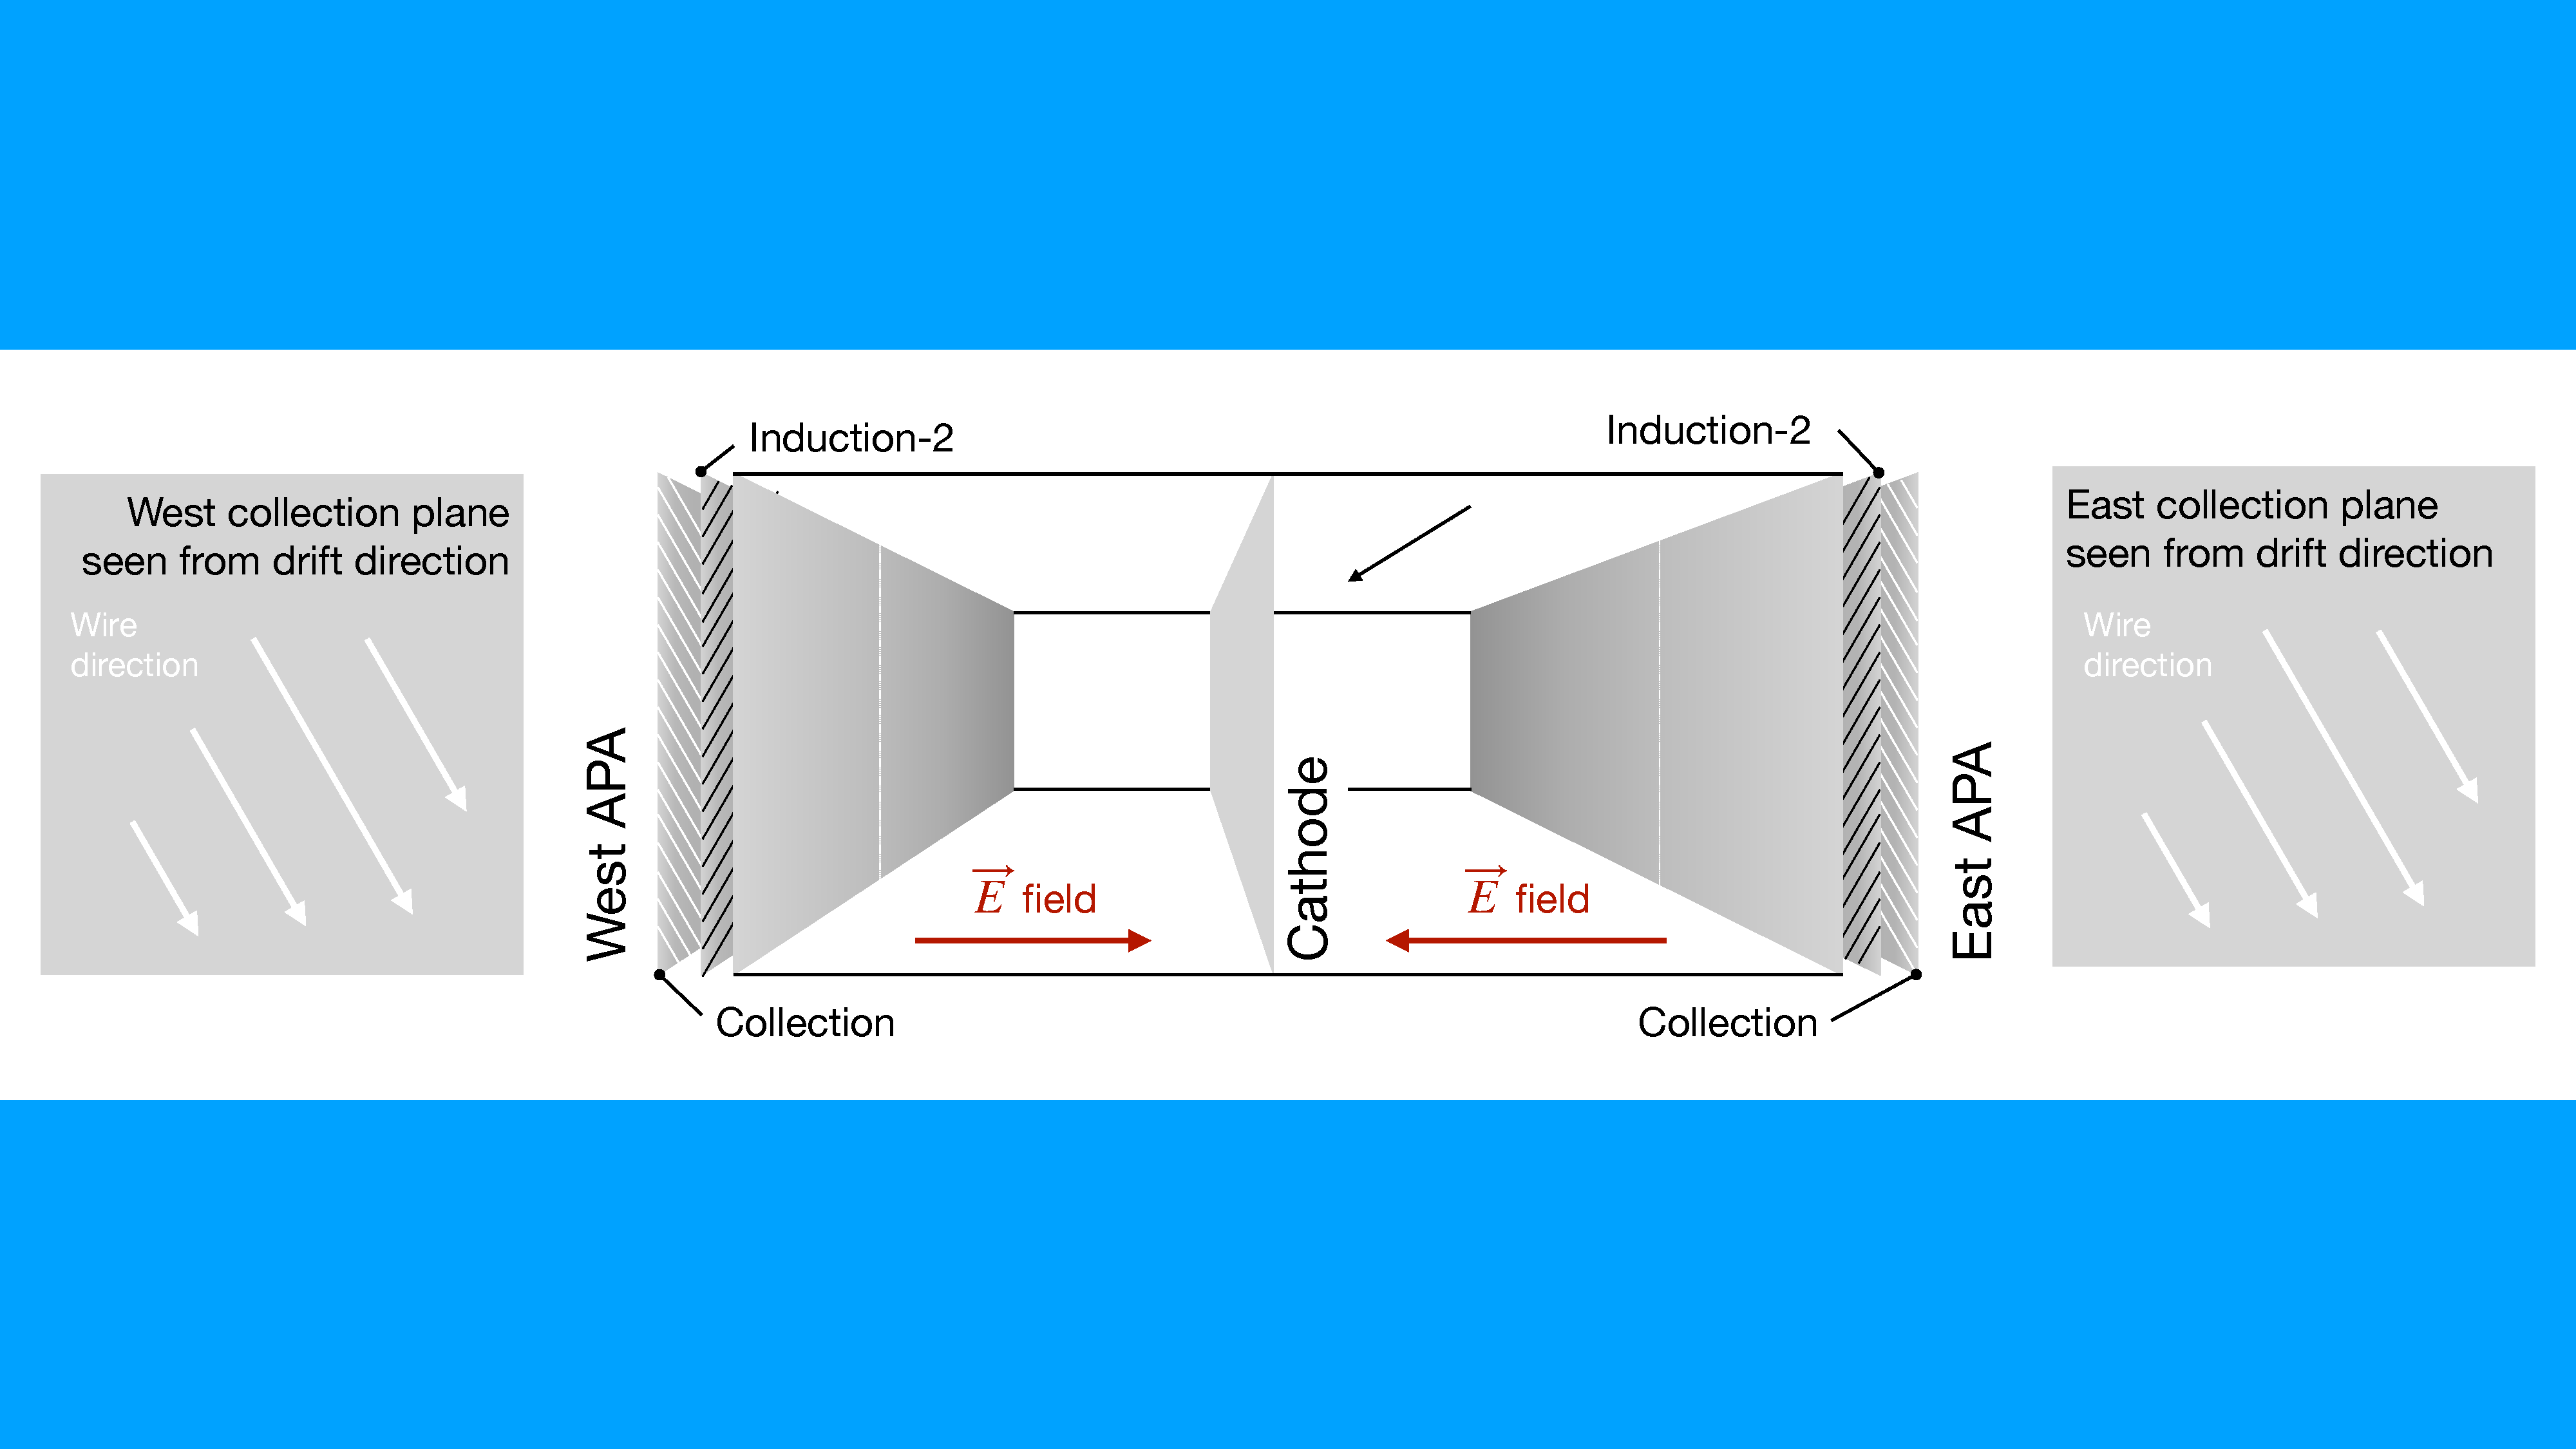
\includegraphics[width=\linewidth, trim={0 9.5cm 0 9.5cm}, clip]{detector/wire_orientation.pdf}
    \caption[T300 module Induction-2 and collection planes wire orientation]{Illustration of the wire direction for the I-2 and C planes for the East and West anode wire planes for each T300 module. The two side panels show the wire direction as seen by an observer located at the central cathode plane and pointing to the drift direction in both TPCs.}
    \label{fig:i2_c_planes_wirepitch_detail}
\end{figure}

In total \num{53248} wires spaced \SI{3}{\mm} apart with lengths up to \SI{9}{\m} across the three planes are installed inside the detector. By appropriately voltage biasing the first two planes (Induction-1 and Induction-2), a non-destructive charge measurement is provided, whereas the full ionisation charge gets collected by the Collection plane. The three planes are kept at $-\SI{250}{\volt}$ (I-1), $-\SI{30}{\volt}$ (I-2) and $+\SI{250}{\volt}$ respectively. The scintillation light is collected by a set of \num{360} PMTs located behind the wireplanes in the APAs. Photos of the installed planes of wires and PMT mounting are shown in \autoref{fig:ICARUS_photo}. 

\begin{figure}
    \centering
    \subfloat[]{\includegraphics[height=5.5cm]{detector/TPC_wires_texts.pdf}\label{fig:ICARUS_wires}}
    \hspace{1em}
    \subfloat[]{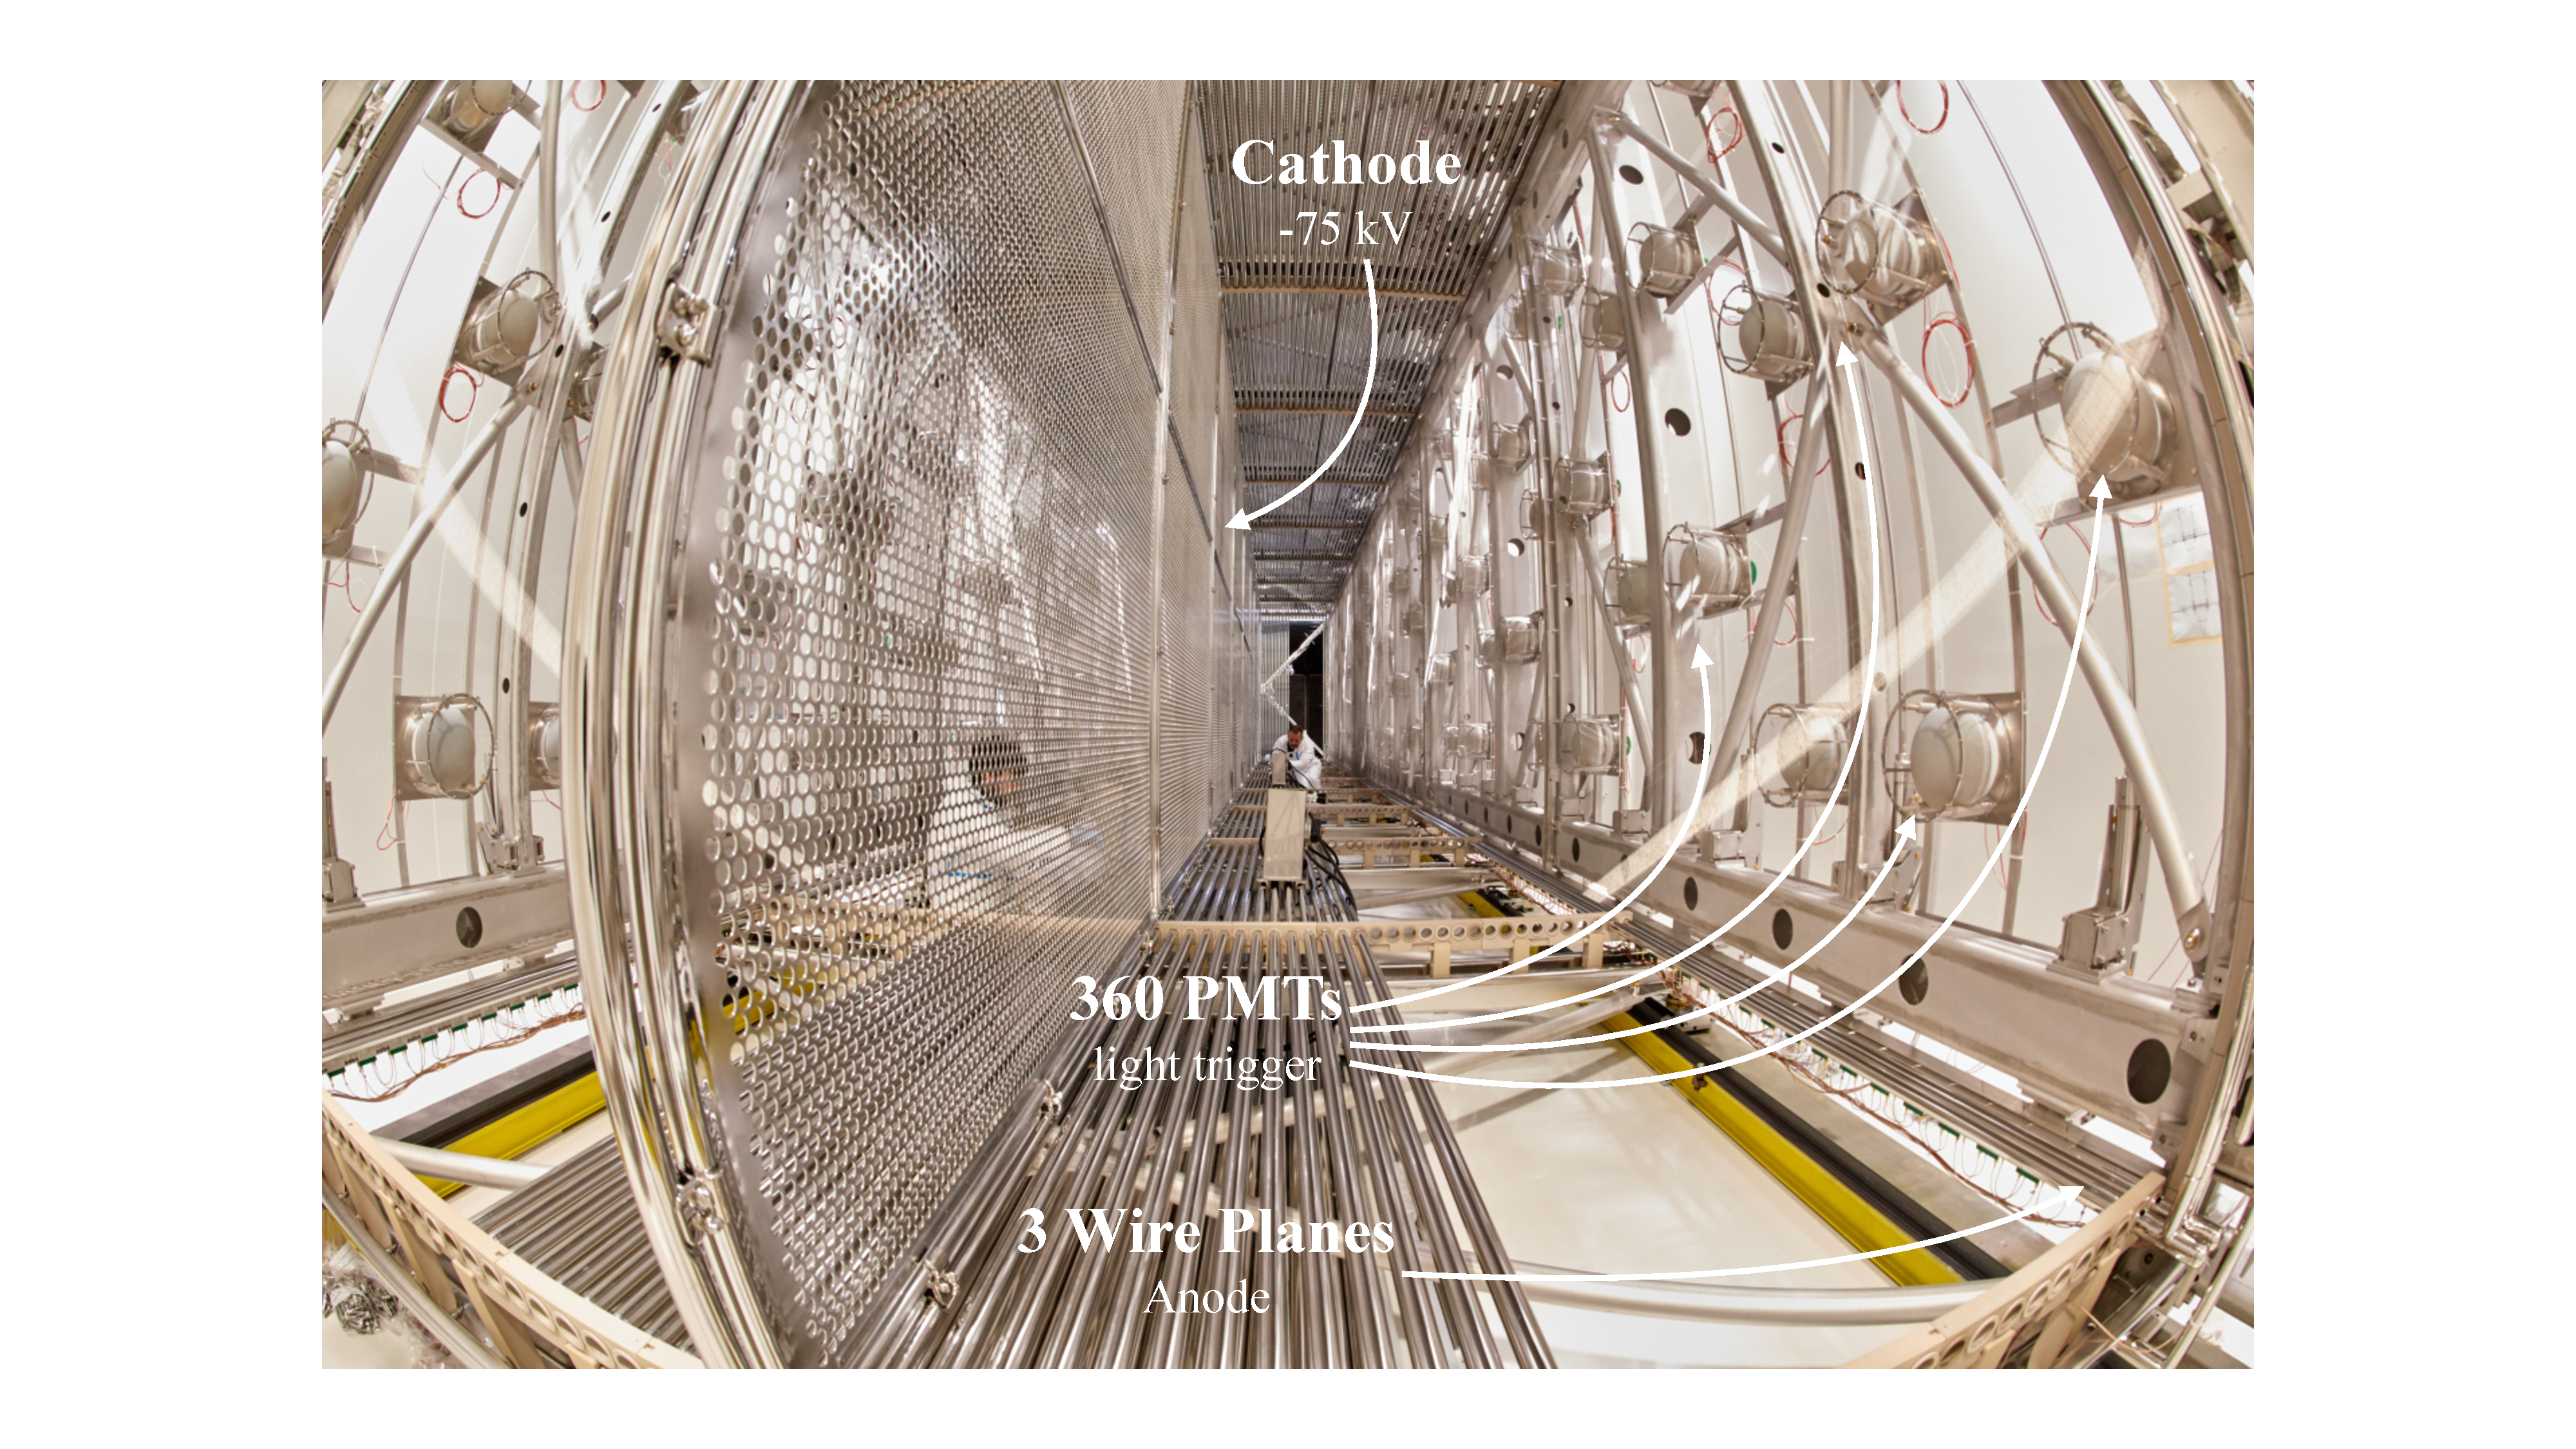
\includegraphics[height=5.5cm, trim={8cm 2cm 8cm 2cm}, clip]{detector/TPC_inner.pdf}\label{fig:ICARUS_PMTs_cage}}
    \caption[ICARUS TPC wires and field cage]{\ref{sub@fig:ICARUS_wires} shows the three planes of wires as installed in the ICARUS detector. \ref{sub@fig:ICARUS_PMTs_cage} shows an inner view of one of the TPCs, with the common central cathode on the left and the anode plane assembly on the right, with the PMTs installed. Figures taken from \cite{amerioDesignConstructionTests2004c,abratenkoICARUSFermilabShortBaseline2023}. }
    \label{fig:ICARUS_photo} 
\end{figure}

The two T300 adjacent modules making up the ICARUS detector are housed inside a warm vessel, in which LN$_2$ is circulated, acting as a cold shield and preventing heat from external thermal insulation from reaching the LAr containers. The external warm vessel uses \SI{60}{\cm} of polyurethane foam to keep argon at its liquid phase just below the boiling point at \SI{87}{\kelvin}. A schematic of the ICARUS detector and the positioning of the two T300 modules is provided in \autoref{fig:ICARUS_scheme}. 

\begin{sidewaysfigure}
    \centering
    \begin{tikzpicture}
        \node at (0,0) {\includegraphics[width=\linewidth]{detector/SBN-FD_composite}};

        \draw[-*, white] (-1,2.5) node [left, white, fill=Gray!15!black] {TPC electronics} -- (0.5,2.25);
        \draw[-*, white] (-9,.5) node [right, white, fill=BrickRed] {Warm vessel} -- (-7.25,-1.5);
        \draw[-*, white] (4,2) node [right, white, fill=Plum!50!black] {Cryogenics} -- (3.25,3.5);
        \draw[-*, white] (7,-0.5) node [below, white, fill=Gray!15!black] {Top-CRT} -- (6.5,4);
        \draw[-*, white] (6,-1.75) node [right, white, fill=Gray!15!black] {Side-CRT} -- (5,-1);
        \draw[-*, white] (6,-3) node [above, white, fill=Gray!15!black] {Bottom-CRT} -- (3.5,-3.75);

        \draw[-*, white] (0,-4.5) node [below, white, fill=Gray!25!black] {East T300 cryostat} -- (-1,-3.5);
        \draw[-*, white] (-4.5,-4.5) node [left, white] {
            \begin{minipage}{4cm}
                \raggedleft
                TPC wireplanes + PMTs
            \end{minipage}} -- (-2.5,-2.5);

        \draw[-Latex, white] (-7,-3.5) -- (-7, -2.5) node[above] {$y$};
        \draw[-Latex, white] (-7,-3.5) -- (-6, -3.2) node[right] {$z$ (beam)};
        \draw[-Latex, white] (-7,-3.5) -- (-7.5, -3.35) node[left] {(drift) $x$};

        \draw[-*, black] (-4.5,5) node [left, black] {\SI{3}{m} concrete overburden} -- (-3,4.5);

        % \draw[step=1.0,white,thin] (-10,-5.5) grid (10,5.5);
        % \foreach \i in {-10,...,10} {
        %     \node [below] at (\i,-5.5) {$\i$};
        % }
        % \foreach \i in {-5,...,5} {
        %     \node [left] at (-10,\i) {$\i$};
        % }

        
    \end{tikzpicture}
    \caption[ICARUS detector illustration]{Illustration of the ICARUS T600 detector at Fermilab. Surrounding the warm vessel is the $4\pi$ coverage CRT. Above the warm vessel, the TPC readout warm electronics are placed, alongside the proximity cryogenics. Inside the warm vessel two identical (east and west) T300 modules are hosted, each containing two TPCs sharing a common cathode at the centre and two anode plane assemblies, one on each side.}
    \label{fig:ICARUS_scheme}
\end{sidewaysfigure}

The ICARUS collaboration successfully collected neutrino interactions during a three-year run at the deep underground laboratories beneath the Gran Sasso Mountains, LNGS (Laboratori Nazionali del Gran Sasso) from 2010 to 2013 \cite{amerioDesignConstructionTests2004c}. The nearly \num{3000} neutrinos collected by the ICARUS detector at LNGS were produced by the CERN to Gran Sasso Neutrinos beam (CNGS) with energy of \qtyrange{10}{30}{\GeV} using protons from the S$\Pp\PAp$S accelerator at CERN. 

The ICARUS detector operating at LNGS demonstrated the superior detection capabilities of the liquid argon TPC design: the detector showed a remarkable $\Pe/\PGg$ separation and particle identification exploiting the measurement of $\dv*{E}{x}$ versus range. The momentum of escaping muons was measured by studying the multiple Coulomb scattering with ${\sim}\SI{15}{\percent}$ average resolution in the \qtyrange{0.4}{4}{\GeV} energy range \cite{ICARUS:2016pvv}. 

LNGS operations demonstrated the feasibility of achieving an exceptionally high level of LAr purity, with a $<\SI{50}{ppt}$ O$_2$-equivalent level of impurities. In 2013 the low-point record of \SI{20}{ppt} O$_2$-equivalent level of impurities was reached \cite{antonelloExperimentalObservationExtremely2014}, corresponding to an exceptionally high electron drift lifetime of \SI{16}{\ms}, marking a milestone for many future experiments, such as the Deep Underground Neutrino Experiment (DUNE). Furthermore, during this period of activity, the ICARUS detector probed the sterile neutrino picture alongside the OPERA detector, providing essential limits toward a better --- tough not definitive --- understanding of the short-baseline neutrino anomaly \cite{antonelloSearchAnomaliesNeappearance2013, antonelloConclusiveConsiderationsComparison2015, agafonovaNewResultsNm2013}. 

From 2015 to 2017 the ICARUS detector underwent a thorough overhaul, first at Laboratori Nazionali di Legnano, Padova (Italy) and then at CERN in the Nutrino Platform framework (WA104/NP01 project), where the TPC electronics were updated to withstand the higher throughput a shallow-depth operation could require, as well as the light collection system and the cryogenic infrastructure. It was then moved in 2018 at Fermilab, where it was placed on the BNB baseline at a distance of \SI{600}{\m} from the source target, operating as the far detector for the SBN program, collecting data from the Booster Neutrino Beam and from the NuMI beam. 

All the ICARUS detector subsystems --- TPC, PMT and CRT --- were commissioned from early 2021 to June 2022, when also the deployment of the concrete overburden was completed \cite{abratenkoICARUSFermilabShortBaseline2023}. This avoids heavy neutral particles entering the TPC volume, resulting in a reduced background activity. 

After the commissioning phase, the first physics data collection run started, lasting until the summer shutdown. Following Run-1, and until the moment of writing, we collected three more physics runs until the recent summer shutdown. The collected/delivered efficiency is estimated to be greater than \SI{95}{\percent}, with a collected exposure of \SI{7.54e20}{POT} for BNB using the FHC mode and a total of \SI{6.35e20}{POT} for the NuMI beam, split between \SI{3.53e20}{POT} in FHC mode and \SI{2.82e20}{POT} in RHC mode. \autoref{fig:BNB_NuMI_POTplot} shows the cumulative POT collected from the start of the ICARUS operations to the present day. 

\begin{figure}
    \centering
    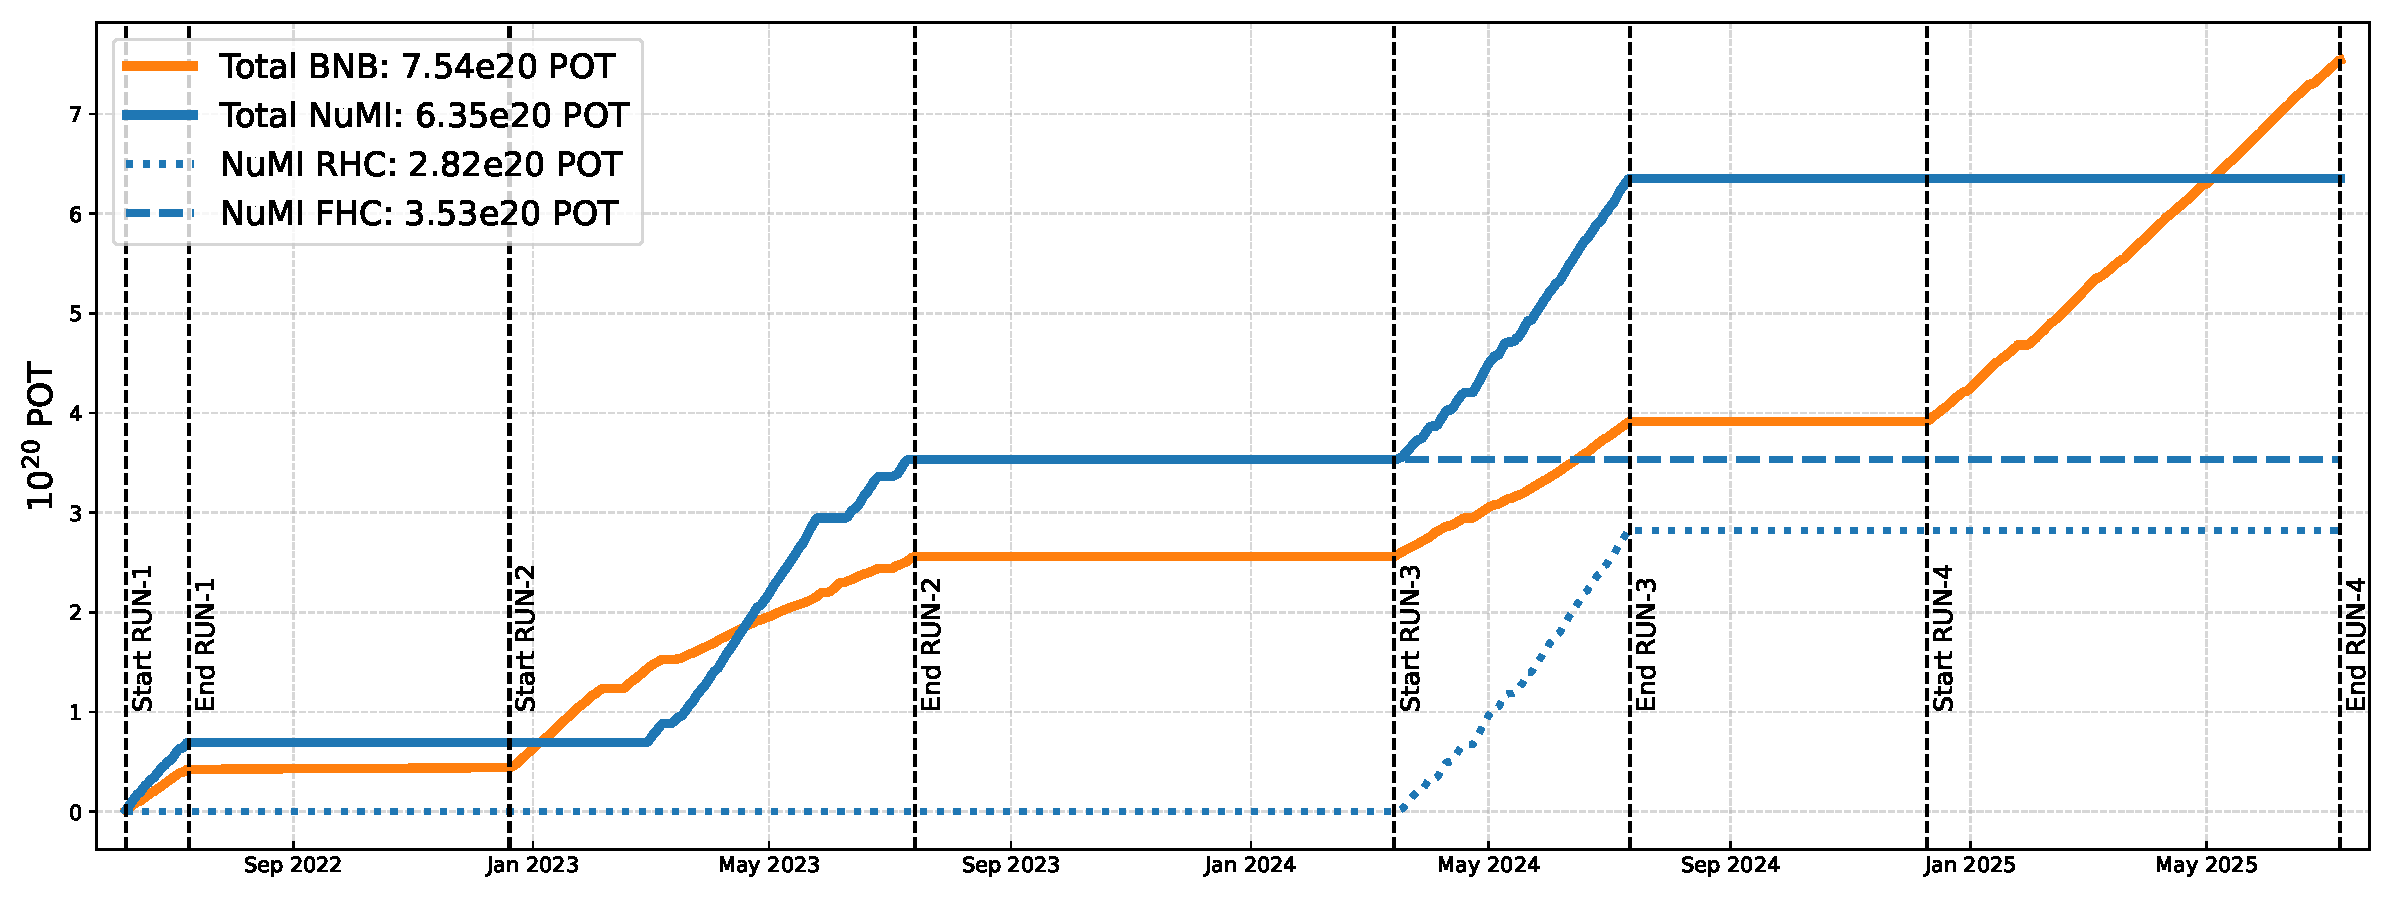
\includegraphics[width=\linewidth]{beams/cumulative_official_runs.pdf}
    \caption[BNB and NuMI collected POT]{Booster Neutrino Beam and NuMI beam proton-on-target collected with ICARUS detector. Courtesy of the run-coordination ICARUS group. }
    \label{fig:BNB_NuMI_POTplot}
\end{figure}

\subsection{The ICARUS detector subsystems} 

All three components (sub-detectors or sub-systems) of the ICARUS detector, upgraded during the detector overhauling process at CERN, are essential for the detector operation and to accomplish its physics goal.

\paragraph{TPC} One of the largest overhauls performed at CERN was the complete redesign of the TPC electronics. During operation at LNGS, the wires were grouped in bunches of 576 wires, read out and filtered to achieve a unipolar signal from all planes. This was convenient in terms of post-processing but showed strong limitations in the case of intense showers \cite{bagbyOverhaulInstallationICARUST6002021}. Such an approach was incompatible with the high rates foreseen for the ICARUS shallow-depth operations at FNAL. The new system combines the previous architecture, which allows for a continuous triggerable multi-buffered waveform recorder for each wire of the detector, with a more advanced design. 

TPC wires are grouped together in bundles of 18 cables and feed through the 96 chimneys positioned above the TPC cryostats. At the other end of the chimneys, the signal is read by the front-end electronics, that are hosted in custom-designed mini-crates mounted on the ultra-high vacuum feedthrough on top of the chimneys. The interface between the TPC wires and the front-end electronics is given by the Decoupling and Biasing Boards (DBBs); each DBB is designed to house two isolated 32-channel banks, allowing each TPC wire to be biased at the proper voltage, enabling proper transparency to ionisation charges, and at the same time preventing parallel noise contributions to wire signal from leakage currents. DBBs are designed to operate in GAr (gaseous argon) and can provide a maximum of \SI{400}{\volt} of voltage bias. The \num{53248} TPC wires are bundled in \num{1664} 32-channel bunches and fed to \num{856} DBBs on the 96 chimneys: on each chimney flange are installed 9 DBBs, serving 576 TPC wires. It is important to note that, while both MicroBooNE and SBND have the TPC readout electronic cold to allow for lower noise RMS, ICARUS has opted to keep its TPC electronic partially warm and thus positioned outside of the TPC cryostat, allowing for easy serviceability. 

The analogue signal is then fed to custom-designed CAEN A2795 boards, housing eight amplifier boards each and capable of integrating and digitising eight channels, for a total of 64 channels for each CAEN board. High throughput is accomplished by employing optical fibre connections in a serial link with a bandwidth of \SI{1.25}{\giga b\per\second}. The digital signal is expressed in units of ADC counts, with the overall TPC electronic giving 1 ADC count per $\sim65\ \Pe$ (or equivalently, $\dv*{Q}{x}\simeq \SI{1000}{ADC\per\cm}$ for a MIP, for which $\dv*{E}{x}\simeq\SI{2.1}{\MeV\per\cm}$).

\paragraph{Light collection system} As mentioned before, once a charged ionising particle crosses liquid argon, ionising it, scintillation light, or VUV photons, is produced from the deexcitation of argon dimers. The light information is crucial for the operation of the ICARUS LArTPC, providing essential information to the event trigger, identifying the interaction occurring in the BNB and NuMI spill gates, as well as calorimetric and position information, useful to complement the 3D track reconstruction by providing absolute timing for each track. 

The ICARUS Light Detection System, or LDS, consists of \num{360} Hamamatsu 8'' R5912-MOD PMTs deployed behind the plane of wires (see figure \ref{fig:ICARUS_PMTs_cage}). Being the PMT glass opaque to the VUV \SI{128}{\nm} light produced by LAr scintillation, they need to be coated with a \SI{200}{\um\per\cm\squared} layer of tetraphenyl butadiene (commonly known as TPB) to convert the VUV light into visible light. 

All PMTs are mounted onto the TPC mechanical frames using a supporting system that allows the PMT to be positioned \SI{5}{\mm} behind the Collection plane. A stainless steel grid cage is mounted around each PMT to mitigate the induction of fake signals on the nearby wire planes by the relatively large PMT signals. The PMTs can be calibrated in time with a laser system based on a Hamamatsu PLP10 laser  diode, emitting laser pulses with $\lambda = \SI{405}{\nm}$ and an FWHM of \SI{60}{ps}, delivered to single PMTs via optical fibres \cite{Icarus:2024dsv}. 

\paragraph{Cosmic ray tagger} Due to its installation at a very shallow depth at the Fermilab BNB baseline, the ICARUS detector is subject to a high rate, ${\sim}10\ \PGm$ tracks per neutrino candidate of cosmic ray-induced interactions inside the detector volume. These particles are one of the primary background components of multiple neutrino physics analyses, as a muon inside the detector volume could be misidentified as the result of a neutrino interaction. The Cosmic Ray Tagger (CRT) is therefore designed to actively address this problem. It fully encloses the detector, covering it from all sides, tagging cosmic muons to clearly identify neutrino interactions. 

It is divided into three parts: the top, side and bottom modules. Each of these modules consists of smaller sixe components to allow for some granularity in the detector, employing the plastic scintillator technology. 

The top CRT is designed to cover the top part of the ICARUS detector; placed just below the \SI{3}{\m} concrete overburden, it intercepts almost \SI{80}{\percent} of the overall cosmic muon flux. It is comprised of 123 detector modules, each with an area of \qtyproduct{1.86x1.86}{\meter}. Each module is made of two orthogonal layers of 8 plastic scintillator bars in which the light is collected by wavelength-shifting optical fibres and read out on both sides by Hamamatsu silicon photomultipliers, enclosed in an aluminium box. The 32 SiPM signals of each Top-CRT module are connected to a CAEN DT5702 Front End  Board (FEB) to produce trigger logic based on  the coincidence between two SiPMs on the same bar and between two layers in a module. 

The side CRT is made using the recovered modules from the MINOS experiment, refurbished with the addition of the SiPM technology to read out the scintillation light.

Finally, the bottom CRT, placed under the detector, is made of 14 modules. Each module was retrieved from Double Chooz experiment and is made of polystyrene strips, and the scintillation light is read out by Hamamatsu PMTs. 

In both side and bottom CRTs the scintillation light is collected by wavelength-shifter optical fibres that are read out by light-sensitive detectors. 

More detailed information about the CRT system can be found in Refs. \cite{ICARUS:2025rdw,Poppi:2023zmp,Poppi:2022vhg}. 